
\documentclass[remotesensing,article,submit,pdftex,moreauthors]{Definitions/mdpi}

%% ---------------------------------------------------------------- metadata
\firstpage{1}
\makeatletter
\setcounter{page}{\@firstpage}
\makeatother
\pubvolume{1}
\issuenum{1}
\articlenumber{0}
\pubyear{2026}
\copyrightyear{2026}
\datereceived{ }
\daterevised{ }
\dateaccepted{ }
\datepublished{ }
\hreflink{https://doi.org/}

\Title{When F1 and ROC-AUC Disagree: A 30-Point Metric Divergence Under
Spatial Interleaving in Extreme-Imbalance Bi-Temporal Change Detection}
\TitleCitation{When F1 and ROC-AUC Disagree: A 30-Point Metric Divergence Under Spatial Interleaving}
\def\orcidauthorA{0009-0000-1260-4504}
\def\orcidauthorB{0009-0001-5418-6096}
\Author{Junzhe Yuan $^{1}$\orcidA\ and Feier Hao $^{2}$\orcidB}
\AuthorNames{Junzhe Yuan and Feier Hao}
\AuthorCitation{Yuan, J.; Hao, F.}
\address[1]{$^{1}$\,School of Environment and Ecology, Hunan Agricultural University, Changsha 410128, China; \newline
$^{2}$\,College of Information and Intelligence, Hunan Agricultural University, Changsha 410128, China}
\corres{Correspondence: haofeier0613@gmail.com}

\graphicspath{{../figures/}{./}}

 \abstract{%
Under extreme class imbalance in bi-temporal mangrove change detection from
Sentinel-2 (change prevalence $0.8$--$2.6\%$), the train/test spatial split
determines which metric a model appears to satisfy. In the single training
region (Vietnam; ${\sim}60$ eligible patches), a spatially interleaved random
split produces a $29.6$-percentage-point higher change $F1$ than a
buffer-separated assignment (positive in all ten partitions; $+11.8$ to
$+32.8$\,pp across ten architectures), while ROC-AUC differs by only $+1.9$\,pp
and prevalence-matched AP by $+15.2$\,pp (six of ten architectures).
A $2\times2$ train/test factorial bounds the prevalence-arithmetic
contribution at ${\sim}9\%$ ($+2.7$\,pp, isolated by reweighting), with the
training$\times$test interaction term ($+17.8$ to $+26.1$\,pp) exceeding
either main effect.
Nine of 90 runs score near-zero $F1$ yet rank at ROC-AUC $0.77$--$0.97$:
under extreme imbalance, a near-zero $F1$ does not imply an uninformative
model. All metrics are agreement with a single noisy reference (GMW); the
$F1$--ROC-AUC divergence is a property of the metric pair under the split
protocol, not a decomposition of model error.}

 \keyword{spatial cross-validation; case prevalence; change detection; extreme class imbalance;
noisy reference labels; buffer separation;
mangrove; Sentinel-2; Global Mangrove Watch; spatially interleaved validation}

%% ---------------------------------------------------------------- document
\begin{document}

\section{Introduction}

Mangrove wetlands occupy less than 0.1\% of the land surface but store
disproportionate amounts of blue carbon, protect tropical coastlines and
sustain estuarine fisheries, while remaining among the fastest-changing coastal
ecosystems on Earth \cite{gmw2018}. Losses are driven by aquaculture conversion
and infrastructure, gains follow restoration and sedimentation, so both
directions matter for policy reporting. Satellite time series are the only
practical way to monitor this consistently across regions, and the 10\,m
resolution and $\sim$5-day revisit of Sentinel-2 (2015--) make it possible to
resolve the narrow, fragmented fringes where most change occurs
\cite{drusch2012sentinel2}.

Deep learning is now the standard tool for bi-temporal change detection
(CD) \cite{shi2020}, and a typical study trains a network on two co-registered
dates and evaluates it on held-out patches drawn from the same scene set. Three
weaknesses follow from that design. First, because patches are extracted on a
stride smaller than their own size, they overlap, so a random patch-level split
puts near-duplicate pixels on both sides; the resulting inflation of spatial
prediction accuracy is a well-documented methodological concern in remote sensing
and ecology~\cite{kapoor2023leakage,ploton2020spatial,roberts2017crossvalidation,valavi2019blockcv}.
Second, the labels for training and testing usually come from one product, so
systematic label error cannot be separated from model error. Third, mangrove
change is extremely rare at pixel level ($0.8$--$2.6\%$ of evaluated pixels
here), and models are rarely benchmarked with metrics that expose the imbalance:
predicting ``no change'' everywhere already reaches binary overall accuracy
0.974--0.992 at the three reference prevalences (four-class OA is a different
denominator and is reported separately).

This study asks a simpler question than ``how much of the gap is leakage?'':
\emph{what does a spatially interleaved random split actually measure?} A
spatially interleaved random split does not measure model capability in
isolation. It measures the joint product of model capability, test-set
composition (including local class prevalence), the spatial train--test
configuration (footprint overlap, near-neighbor proximity, local morphology),
and the metric's sensitivity to those factors. A high $F1$ under an interleaved
split is therefore an \emph{evaluation-protocol-dependent quantity}, not a pure
estimate of detection ability. Three sub-questions structure the paper.
First: \emph{is the difference a model effect or a protocol effect?} The
model suite---ten architectures and two pixel baselines---is a controlled
variable, not an object of comparison; only the split assignment varies.
The phenomenon is consistent in direction across all ten
architectures (secondary evidence, given the shared training data and recipe),
consistent with a protocol-level effect. Second: \emph{which parts of the score are model capability,
and which are properties of the evaluation design?} The answer is bracketed with
three metrics of different prevalence sensitivity and a factorial that
identifies a measurable test-composition component. Third: \emph{which
components can be identified, and which remain confounded?} A matched-prevalence,
zero-overlap control at reduced patch geometry shows the spatial-position
contrast is not detectable (underpowered; effective $n{=}5$).
The reduced-scale block control is negative in sign but its magnitude is
unidentified. The individual contributions of overlap, proximity, and morphology
at the original geometry remain jointly confounded. Models are trained on the Red River Delta (Vietnam) and tested, with no
fine-tuning, on two geographically disjoint Chinese sites, with a second
Sentinel-2-based reference product as an extent-level label-source sensitivity check.

Two of the mechanisms this configuration can carry are worth naming,
because the distinction is the one the whole paper turns on.
\emph{Level-1 direct overlap}: test patches share at least one pixel with
a training patch, so near-duplicate observations appear on both sides of
the split. This is an artefact of the sampling geometry, is absent from
every deployment, and needs no inference to establish---30 of 30 test
patches in the primary interleaved protocol and 98 of 100 in the
secondary one share a pixel with the training set. \emph{Level-2
residual proximity}: even with no shared pixel and a guaranteed geometric
gap, test patches near the training region share kilometre-scale
landscape context (mangrove texture, tidal regime, sediment and coastline
morphology) that a model may legitimately exploit at deployment.

The contributions are three. First, a quantified $F1$--ROC-AUC divergence
under extreme imbalance: spatially interleaved and buffer-separated evaluation
produce a $29.6$\,pp difference in change $F1$ (positive in all ten
partitions, $+11.8$ to $+32.8$\,pp across ten architectures) while ROC-AUC
differs by only $+1.9$\,pp and prevalence-matched AP by $+15.2$\,pp
(Sections~\ref{sec:rand} and~\ref{sec:metric}). Second, a $2\times2$
train/test factorial bounding the prevalence-arithmetic contribution at
${\sim}9\%$ of the gap ($+2.7$\,pp;
$+2.7$ to $+9.6$\,pp across orderings, isolated by reweighting), with the
training$\times$test interaction term ($+17.8$ to $+26.1$\,pp,
$60$--$88\%$ of the total) exceeding either main effect, and neither
assignment alone contributing more than $+11.4$\,pp
(Section~\ref{sec:prevalence}). Third, a demonstration that nine of 90 runs
score near-zero $F1$ yet rank at ROC-AUC $0.77$--$0.97$: under extreme
imbalance, a near-zero $F1$ does not imply an uninformative model, and
reporting $F1$ alone misrepresents the model's information content
(Section~\ref{sec:metric}).

Prior work has established that spatially independent splits are required for
honest evaluation~\cite{roberts2017crossvalidation,valavi2019blockcv}, and that
spatial prediction accuracy is
inflated when training and test patches overlap~\cite{ploton2020spatial}. The
incremental contribution here is the quantification of the $F1$--ROC-AUC
divergence under extreme class imbalance ($0.8$--$2.6\%$ change prevalence) in
a bi-temporal deep-learning setting, with an explicit factorial decomposition (Section~\ref{sec:prevalence})
and an identification boundary statement (Section~\ref{sec:boundary}).

A reporting checklist (Section~\ref{sec:checklist}) distils these findings
into practical checks for single-region change-detection studies. The paper makes
no architecture ranking, no field-accuracy claim, and no causal
decomposition of the residual contrast.

\subsection{Related Work}

Bi-temporal change detection has moved from post-classification comparison to
end-to-end two-encoder architectures~\cite{daudt2018siamese,chen2021dasnet} and,
more recently, to attention and Transformer backbones~\cite{bandara2022changeformer}.
These are typically benchmarked on random in-region splits, which, as shown here,
re-use the spatial shortcut that spatial autocorrelation
provides~\cite{ploton2020spatial,zhan2026leakage}. For mangroves specifically,
the literature is still dominated by in-region evaluation. U-Net-based
extent classification~\cite{maung2023wunbaik} and deep-learning change
detection over 1990--2024~\cite{win2024wunbaik} report high
accuracies on in-region samples; multi-method spectral-index and
object-based change detection~\cite{fu2023beibu,son2015camau} predate the
deep-learning era. None of these measures transfer to a geographically
disjoint region, nor do they report the cost of the split they use.

The accuracy-assessment literature makes the methodological point within which
these results sit. Olofsson et al.~\cite{olofsson2014accuracy} set out how area and
accuracy should be estimated from a probability sample with a spatially explicit
design rather than from a convenience sample of pixels; Meyer and
Pebesma~\cite{meyer2021aoa} show how little of a mapping product can be validated
outside its area of applicability. Karasiak et al.~\cite{karasiak2022spatial}
compare spatial and non-spatial resampling for the same task.
Spatial leave-one-out, with a buffer radius set from a Moran correlogram,
yields unbiased predictive error; non-spatial splits overestimate it.
The sharper point: block, object, or cluster partitioning at a fixed distance
\emph{assumes} the dependence has been removed without checking, so residual
dependence may persist. Kattenborn
et al.~\cite{kattenborn2022spatial} show that spatially autocorrelated
train/validation samples directly inflate model accuracy, but do not
decompose the inflation into footprint overlap versus residual proximity,
which is the factorial contrast attempted here; Wadoux et
al.~\cite{wadoux2021spatialcv} argue that spatial cross-validation is a
model-development tool rather than a route to design-based accuracy
estimation, which is why agreement with a reference is reported rather than
absolute accuracy; Wang et
al.~\cite{wang2023spatialplus} propose a new spatial CV method that explicitly
accounts for spatial structure, and Stock~\cite{stock2025blocks} provides
practical guidance on block-size selection for spatial CV in remote
sensing, demonstrated on synthetic data mimicking a marine application; Mil\`a et
al.~\cite{mila2022nndm} match the test--training distance distribution to
that of the target prediction area, and how far a buffer of practical size falls
short of the spatial separation they recommend is measured; de
Bruin et al.~\cite{debruin2022clustered}
show that cross-validation accuracy for spatially clustered samples needs a
resampling design that respects the clustering. Their premise is confirmed:
separation removes shared footprints but not statistical independence, because
the change label itself is coherent over $1$--$2$\,km.
The distance response under the buffer-separated split is descriptive, not
significant (Section~\ref{sec:geom}). Spatial block
  cross-validation for
  structured data~\cite{roberts2017crossvalidation,valavi2019blockcv} is the
  resampling lineage followed here. Concurrent work has shown that spatial
  domain mismatch between reference sources inflates apparent model accuracy
  in biomass estimation~\cite{hasoba2026domain}; the same principle
  operates in bi-temporal change detection, where the mechanism is train/test
  spatial proximity rather than sensor-domain difference. Recent land-cover
  change detection work reports that spatially-blocked CV yields lower accuracy
 than random CV~\cite{manikandan2026foundation}. The contribution here is the
factorial decomposition of the inflation into prevalence arithmetic and a joint
spatial-configuration component, with a direct reweighting that
measures the prevalence term on its own.
The same inflation has been documented in other
domains~\cite{kumar2025randomcv}.

A separate body of work establishes that, under class imbalance, the
precision--recall operating point is more informative than the ROC operating
point~\cite{saito2015precision} and that the two metrics respond differently
to prevalence shifts~\cite{davis2006relation}. Those results answer the
question \emph{which metric to report}. The question addressed here is
different: given a fixed model and a fixed metric pair, \emph{how large a
divergence between $F1$ and ROC-AUC can the evaluation protocol itself
manufacture}, and how that divergence decomposes into prevalence arithmetic
versus a joint spatial-configuration component. The protocol is the
independent variable; the metric divergence is the dependent variable.

 \section{Study Areas and Data}
\subsection{Study Areas}

Three estuarine/coastal mangrove areas with contrasting change trajectories
were selected after verifying their extent against Global Mangrove Watch
(GMW): the Red River Delta, Vietnam (106.50--107.00$^\circ$E,
20.50--21.20$^\circ$N), used for training; the Beilunhe estuary, Guangxi, China
(108.10--108.70$^\circ$E, 21.15--21.75$^\circ$N); and Zhanjiang, Guangdong,
China (110.05--110.85$^\circ$E, 21.00--21.50$^\circ$N), both used only for
testing. The two test sites lie in different river estuaries in China,
$\sim$180--390\,km from the training site. The training site lies in UTM zone
48N; both test sites in 49N. The Beilunhe \emph{tile} set straddles 108$^\circ$E
and spans both zones. The mosaic is built by reprojecting the
zone-48 tiles onto the zone-49 grid; agreement with the natively
zoned tiles is 99.2\% of pixels in Beilunhe and 99.8\% in Zhanjiang.
The zone-48 contribution is a 0.435\% sliver of the Beilunhe window, touched by
none of the 18 retained patches. According to the GMW v4.1.12 layers, mangrove extent
changed from 77.4 to 70.9\,km$^2$ in the training region (13.4\,km$^2$ loss,
6.9\,km$^2$ gain), from 18.3 to 19.0\,km$^2$ at Beilunhe and from 14.6 to 19.1\,km$^2$ at Zhanjiang between the nominal 2019 and 2024 GMW endpoints. These are
differences between two \emph{reference} layers, not estimates of change
accuracy. Decomposing the disagreement separates its two causes: holding the
year fixed, swapping the v4.1.12 extent layer for the differently-sensored
v4.0.19 one accounts for 19.8 / 3.6 / 7.3\,km$^2$, while holding the source fixed, one
nominal year of revisit accounts for only 4.6 / 0.3 / 1.0\,km$^2$. Measured
against the net extent change above (6.5 / 0.7 / 4.5\,km$^2$), the inter-source
term is 1.6--5.1 times the signal it is used to measure and the revisit term
0.2--0.7 times. The disagreement between two
references is therefore larger than the change signal, not a small perturbation
of it, which is why no confidence interval is attached to these numbers and they
are not used as an area inventory. Figure~\ref{fig:split} shows
the regional layout and the spatial split.

\begin{figure}[H]
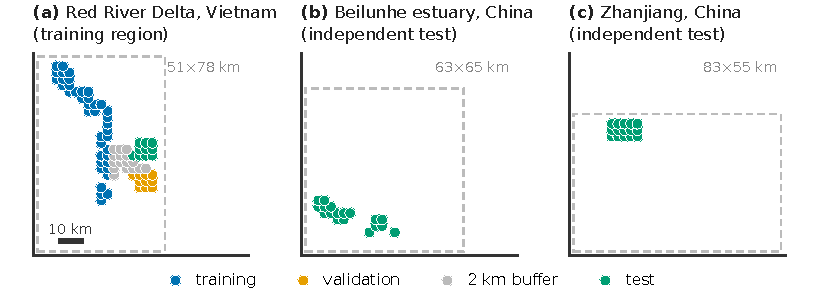
\includegraphics[width=\textwidth]{fig1_spatial_split.pdf}
\caption{Study regions and spatial split. Training patches are taken only from
the western/central part of the Red River Delta box; a 2\,km buffer separates
them from the validation/test zone. Beilunhe and Zhanjiang are test regions
never seen during training, and geographically disjoint from the training zone.
(a) Red River Delta, Vietnam (training region; 40 training, 10 validation,
16 buffer and 10 test patches); (b) Beilunhe estuary, China (18 test patches);
(c) Zhanjiang, China (15 test patches). The three panels share one scale --- the
scale bar applies to all of them --- and the grey dashed rectangle in each is the
region footprint, labelled with its extent.}
\label{fig:split}
\end{figure}

\subsection{Sentinel-2 Dry-Season Composites}
\label{sec:composites}

Level-2A Sentinel-2 tiles came from the AWS Open Data Sentinel-2 L2A COG
collection, which serves a single offset-free $0$--$10000$ digital-number scale.
No $-1000$ bottom-of-atmosphere offset is applied by that product; 99.99\% of
$t_2$ values over a deep-water tile pair lie below $1000$. The
two epochs ($t_1$: Dec 2019, $t_2$: Dec 2024) span the Sentinel-2 L2A
processing-baseline revision of January 2022, which introduced a $+1000$
BOA offset in the official product. The AWS COG collection appears to
serve both epochs on the same scale; tile-by-tile STAC verification
confirms the underlying products use different processing baselines
($t_1$: 02.13/05.00, $t_2$: 05.11), so the common scale is a property of
the COG reprocessing, not of the original L2A product. No cross-epoch
radiometric harmonisation is applied.
A residual additive or multiplicative bias between epochs cannot be excluded,
and unharmonised temporal radiometric variation is treated as an unresolved
nuisance factor rather than a resolved property.

Two independent checks on the actual composites (Appendix~\ref{app:repro}) give
a directionally consistent but non-quantitative check (no reverse power). Water, the standard pseudo-invariant
target, agrees closely in the training region: the 95th percentile of
water pixels differs by under $1\%$ in the near-infrared and short-wave bands
($2666$ against $2658$ in B08) and by $5$--$8\%$ in the blue and green bands.
At the two test sites the same blue and green bands differ by $8$--$15\%$. A
pseudo-invariant-feature regression over stable vegetation does \emph{not}
return unit gain: fitted gains span $0.34$--$0.94$ with correlations of
$0.35$--$0.77$. This is not read as proof of a radiometric mismatch.
The target is not invariant across a five-year interval of real mangrove change,
and tiles were averaged on differing grids before comparison.
Both factors bias the slope away from one. It does mean that the absence of
harmonisation rests on the water-target check alone, which is weaker than a
cross-sensor harmonisation would require, and a residual additive bias between
epochs cannot be excluded. The $0.34$--$0.94$ gain range implies that, if a true
radiometric drift exists, its direction and magnitude are unknown and could
either amplify or attenuate the measured change signal. This is stated as a
limitation of the change labels, rather than as a claim that the two epochs are
radiometrically interchangeable. Two dry-season windows were used: 1 December 2019--31
January 2020 ($t_1$) and 1 December 2024--31 January 2025 ($t_2$); dry seasons
minimise cloud and the tidal differences that otherwise dominate mangrove
spectra.

Scene selection used the Scene Classification Layer over the region window
rather than tile-level cloud metadata, which was found to be a poor proxy for
cloud over a small window. Following the ESA codebook, SCL 1--7 are treated as
clear---1 saturated or defective, 2 dark-area pixels, 3 cloud shadows,
4 vegetation, 5 not-vegetated, 6 water, 7 unclassified---and exclude class~0
and the cloud family 8--11 (there is no class~12). Inside the window, class~1
is absent from all 40 scenes, class~2 (dark) contributes at most $2.0\%$ and
class~3 (shadow) at most $9.4\%$, and the
retained class~7 (unclassified, which can include medium-probability cloud)
reaches $17.1\%$. Non-clear pixels are zero-filled; realised zero-fill is
$\leq$0.4\% of any patch and the $t_2$ Vietnam composites have no holes. Two
scenes were greedily selected per tile-epoch subject to a mangrove clear
fraction $\ge\,0.60$ and a region clear fraction $\ge\,0.50$, giving 40 scenes
over 20 tile-epochs; per-scene dates, tidal labels and clear fractions are in
Table~\ref{tab:scenes}.

Two properties of that selection limit what the composites can support, and
they are stated here rather than in the limitations. First, each tile-epoch
contributes exactly two scenes, so the per-pixel median is a mean of two and
cannot suppress single-scene contamination. Per-scene mangrove clear fractions
range from $0.74$ to $1.000$ across the 40 scenes. The four Vietnam $t_2$ tiles
are the low end at $0.74$--$0.85$; the 2024-12-05 pair is the cloudiest,
with whole-tile clear only $0.49$--$0.71$.
Second, tidal state---assigned coarsely from lunar age, not measured---is
\emph{not matched} between epochs: $t_1$ mixes spring and mid states while $t_2$
is almost entirely mid, and Zhanjiang in particular pairs a spring/neap $t_1$
with a mid/neap $t_2$. Because whether a fringe pixel counts as change depends
on what was exposed at acquisition, some part of the fringe signal may be water
level rather than vegetation. Tide-gauge or altimetry data could not be obtained
for these windows, so this confound is stated and not corrected. The label is
also not comparable across basins: the Gulf of Tonkin and the Beibu Gulf differ
in tidal regime, so a given lunar-age label corresponds to a different water
level in the Vietnam training region than in the two Chinese test regions. Each
tile-epoch was composited to a per-pixel median of the clear observations, 20\,m
bands were resampled bilinearly to 10\,m, and the feature stack is
[B02, B03, B04, B08, B11, B12, NDVI, NDWI, MNDWI].

\subsection{Change Labels and the Second Label Source}
\label{sec:labels}

Training and primary test labels come from GMW v4.1.12, a global
mangrove extent time series. The GMW consortium reports a global
mangrove-extent F1 of 0.928 (omission 6.4\%, commission 8.1\%), estimated
against 32{,}569 reference points at 120 sites~\cite{gmw2024v4}; that figure
characterises extent delineation, not change delineation, and the consortium
publishes no equivalent summary for the change classes. It is quoted as context
for the \emph{reference quality}. It is not a bound on the model--reference agreement
metrics reported here. Those metrics measure agreement with GMW, which can
approach unity even where GMW itself deviates from the ground truth.
A model can score poorly against the reference while tracking the ground truth
more closely than the reference does. The 2019 and 2024 layers were intersected to produce
a four-class change map: \emph{stable mangrove}, \emph{loss}, \emph{gain},
\emph{stable background}. Labels were reprojected from the native GMW grid
(WGS84, $0.000269^\circ$, about 30\,m) onto the 10\,m UTM image grid
(nearest neighbour). The two grids do not tile in an exact integer ratio:
source-cell boundaries do not coincide with the 10\,m pixel grid and shift a
few pixels at each boundary. This is treated explicitly as a source of
boundary error (Section~\ref{sec:discussion}).

As a second label source, the GMW 2020 layer v4.0.19
(Zenodo record 12756047) is used, produced from Sentinel-2 imagery with a different
classifier. It is a \emph{same-family, differently-sensored estimate of the same
mangrove extent}---a label-source sensitivity check, not independent ground
truth---and because it is a one-year extent map it can
score the \emph{presence} class only, never the change class. One degree tile of
that release (20--21$^\circ$N, 108--109$^\circ$E) is absent but intersects none
of the three study regions, so coverage is complete in all of them.

\subsection{Patch Extraction and the Spatial Designs}
\label{sec:split}

Patches of 512$\times$512 pixels (5.12\,km) were extracted on a 256-pixel
stride, keeping those with a mangrove fraction of 5--85\% (union of both epochs)
and a clear fraction $\ge$\,0.6 in both epochs: 76 patches in the training
region, 18 at Beilunhe, 15 at Zhanjiang. All metrics are computed on this
filtered subset, not on the full regional extent. Inside the training region the
grid was split into three column zones---training, a buffer, and a
validation/test zone---with the buffer discarded, so that no training patch is
closer than 2\,km to any validation/test patch. On the 256\,px grid the
achievable edge distances are multiples of 2.56\,km, so the nominal 2\,km
guarantee realises as 2.56\,km (Section~\ref{sec:rand}). The 76 patches resolve to 40
training, 10 validation and 10 test patches, 16 falling in the buffer and never
used; validation and test are further separated by a row buffer. Early stopping
uses the validation zone alone, which is separated from the test zone, so model
selection does not bias the within-region numbers. Note that this is a
\emph{sampling-separation} guarantee only: patches overlap 50\% on the
extraction grid and the landscape is continuous, so separation does not imply
statistical independence---a distinction this paper measures rather than assumes.
Table~\ref{tab:data} gives the data volumes.





% ===== END AUTO-GENERATED by analysis/make_supplementary_tables.py =====



\section{Experimental Design}
\subsection{Task Formulation}

Let $X_1, X_2 \in \mathbb{R}^{H\times W\times 9}$ be the two feature stacks.
The network predicts, for every 10\,m pixel, one of four classes
$\mathcal{C} = \{\text{stable mangrove}, \text{loss}, \text{gain},
\text{stable background}\}$. Change is the union of \emph{loss} and
\emph{gain}. Framing the task as a single four-class segmentation (rather than
two binary problems) lets one network exploit the shared spectral signature of
mangrove presence while still separating the two change directions. The task
is \emph{endpoint change} between the two seasonal composites: a pixel is
loss (gain) if the reference classifies it as mangrove at $t_1$ but not at
$t_2$ (the reverse). Intermediate dynamics (loss followed by regrowth within
2019--2024) are invisible to this formulation and are labelled stable.

\subsection{Model Suite as a Controlled Variable}
\label{sec:arch}

A fixed suite of ten deep networks was trained under one protocol---identical
data, spatial splits, loss, schedule, optimiser and hyper-parameters---spanning
an encoder--decoder family with and without convolutional block
attention~\cite{ronneberger2015unet,woo2018cbam} and a multi-scale feature gate,
a dilated-backbone segmentation model~\cite{chen2018deeplabv3plus} with and
without ImageNet initialisation, two dual-encoder variants that consume the two
dates separately, and one lightweight Transformer (specification in
Table~\ref{tab:archspec}).
The architectures are a \emph{controlled variable}, not an object of
comparison: the design priced in Section~\ref{sec:rand} is applied identically
to all of them, so a result that holds for all ten cannot be an artefact of one
architecture. No architecture ranking is therefore attempted, and the residual
architecture-level variation is reported as an
observation with its spatial fragility stated, not as a resolved ordering.

It should be stated explicitly which standard baseline families are \emph{absent},
because their absence is a scope decision rather than an oversight. The suite
contains no CVA/index-difference fusion variant, no BIT-style
bidirectional-image-transformer, no SNUNet-style densely connected nested U-Net,
and no encoder pretrained on remote-sensing imagery (the only pretrained-encoder
control is supervised on ImageNet, not on remote sensing). The one non-deep
reference, the post-classification comparison introduced below, classifies each
date independently rather than differencing bands or indices, so it does not
cover those families either. They were not added, and the numbers here are not
read against published state of the art on the common change detection benchmarks.
This is a scope limitation: the per-architecture numbers in
Table~\ref{tab:main} are not comparable to published benchmarks that include
these families. The reason is the object of this paper: those published
scores are obtained under patch- or image-level splits whose geometry is shown
here to move within-region change $F1$ by tens of points, so aligning the split
here with theirs to make the comparison legible would reintroduce the confound this
paper exists to price. What the suite is for is holding the architecture fixed
while the split varies, and the ten deep networks spanning six families and
$2.3$--$19$M parameters (enumerated in Table~\ref{tab:archspec}) are already more
than that argument needs; a design effect that reproduces across all of them is not
waiting on an eleventh. A reader whose question is \emph{which architecture is
best on this data} should treat this paper as not answering it.

Three deviations bound what the suite can be used for. The dual-encoder models
consume $X_1$ and $X_2$ separately while the static models receive the
27-channel concatenation $[X_1, X_2, |X_1-X_2|]$, so input representation is
confounded with architecture; the FC-Siam implementation uses two encoders with
\emph{separate} weights, whereas both Siamese variants of
Daudt et al.~\cite{daudt2018siamese} share weights and differ only in how the
skip connections are done, so ours is a two-encoder variant
and is labelled as such; and the Transformer is re-designed from scratch,
\emph{inspired by} ChangeFormer~\cite{bandara2022changeformer} but using neither
its hierarchical transformer encoder and MLP decoder nor any pretrained
weights, so its failure
($F1_{ch}$ 0.01--0.02) is evidence about the implementation and not about the
ChangeFormer architecture.

Two non-deep references bracket the suite. The pixel-level baselines
(Section~\ref{sec:results}) are effectively useless on the change classes. A
post-classification comparison (PCC) baseline---a plain U-Net classifying each
epoch independently into presence/absence, with change defined as
disagreement between the two class maps---is now reported under both
protocols. At Zhanjiang it reaches change $F1$ $0.40$ (three-seed mean,
$0.40/0.40/0.40$) under the primary uniform scheme and $0.41$
($0.44/0.40/0.40$) under the secondary square-root scheme. Against the best
deep model (FC-Siam) under the \emph{same} scheme, the ordering flips by
protocol---$0.40$ versus $0.43$ under uniform, $0.41$ versus $0.38$ under
square-root---but the two are within three points in both cases. This is read
as evidence that the choice of formulation (PCC versus deep) is not the
consequential variable here, not as a claim about the two formulations
(Appendix~\ref{app:repro}).

\subsection{Training and Class Imbalance}
 \label{sec:train}

All models were trained with PyTorch 2.14.0 on one RTX 4080
Laptop GPU (12\,GB), one model at a time. The nine-band stack is stored on a
single 0--10000 scale and divided by $10^4$; the three indices $\mathrm{NDVI}$,
$\mathrm{NDWI}$ and $\mathrm{MNDWI}$ are stored as $(x+1)\cdot5000$, so all nine
channels share one non-negative range. No alternative scaling was tested, and
this is treated as storage convenience, not an optimisation result. The recipe is Adam
(learning rate $10^{-3}$, weight decay $10^{-4}$), a cosine schedule, batch size 8
(2 for the dual-encoder temporal models, which do not fit two 512\,px stacks in
12\,GB), up to 100 epochs, and early stopping with patience 15 on validation
mIoU; most runs converge within 25--40 epochs. Early stopping on a
background-dominated metric is a choice that would be revised. Augmentation is random
$90^\circ$ rotation and horizontal flip, applied identically to both dates and the
labels. The loss is class-weighted cross entropy plus a soft multi-class Dice
term at 1:1, the Dice computed over the sum of all four classes (so background
contributes most of its gradient) and including the background class. The Dice
term was essential: with weighted cross entropy alone the two smallest
architectures reached zero change $F1$---which overall accuracy does not
reveal. As a control for the batch-2 temporal model, the
same architecture was also trained with GroupNorm(8) in place of BatchNorm,
isolating the normalisation component but not the optimisation-trajectory
component.

Change pixels are 0.8--2.6\% of evaluated pixels in the two Chinese test
regions, $3.9\%$ in the training region (full Vietnam tile; the 76 training
patches carry $2.84\%$) and $2.9$--$3.8\%$ in the interleaved test draws.
Class weights matter~\cite{chen2025classimbalance}. Three
schemes are pre-specified: inverse frequency $w_c=1/(4f_c)$ (which gives the
rare gain class roughly $58\times$ the weight of background), square-root
$w_c=1/(4\sqrt{f_c})$ (about $7.6\times$), and uniform $w_c=1$. Two
training-region-only protocols select among them before any test outcome is
seen: a validation-zone mIoU rule on three matched U-Net probes, which selects
square-root (0.462 against 0.453 uniform and 0.443 inverse), and a nested spatial
3-fold CV on the training zone alone, which selects uniform (0.535 against 0.531
and 0.528)~\cite{roberts2017crossvalidation,valavi2019blockcv}. The
between-scheme spread (0.007) is six to seven times smaller than the
between-fold spread (0.045), so the two protocols are statistically
indistinguishable rather than in genuine disagreement; a
tie-break (uniform) is pre-specified. No scheme is designated optimal and weights
are not tuned per region.

Pixel-level baselines use the same nine-band stacks as 27 features ($t_1$,
$t_2$, $|t_1-t_2|$), a random subsample of at most 300\,000 training pixels,
default hyper-parameters (Random Forest 300 trees, SVM RBF $C=1$), and each is
trained both unweighted and with balanced class weights, so the
deep-versus-pixel comparison is not an artefact of a weakened baseline. Their
low change $F1$ ($0.016$--$0.197$ unweighted) reflects heavy under-sampling of
the rare class rather than a limit of the model family, and they are read as
applying to this fixed configuration only.

Re-running U-Net+CBAM+MSA end-to-end in deterministic
mode (deterministic cuDNN/cuBLAS, fixed RNG, a cross entropy composed from
deterministic primitives, with a warn-only relaxation for CBAM adaptive
max-pooling) reproduces every reported metric bit-identically; a repeat in
default mode differs by at most $0.013$ in $F1_{ch}$, about a third of the
seed-to-seed standard deviation (0.041). GPU non-determinism therefore does not
affect the reported means or the seed-based inference built on them.

\subsection{The Evaluation-Design Experiment Suite}
\label{sec:geom}

 The seven experiments below are treated as one internally pre-specified suite, and each
is registered before it is reported: for every experiment the question, the
units, and the known confounds are stated, so that
every claim in this paper is traceable to a row of that registration. The cards
themselves are given in Appendix~\ref{app:reg}.

 Two geometric facts that all seven experiments depend on are stated up front.
 Patches are 512\,px on a 256\,px stride, so a set of $n$ patches covers between
 $n$ and $4n$ distinct footprints. The ratio of summed to distinct area is called
 the \emph{duplication factor}: 2.22 for the Vietnam test zone, 1.85 for
 Beilunhe, 2.50 for Zhanjiang, at most 4 everywhere. Because the
 buffer-isolated (honest) zones are contiguous while the interleaved random test
 patches are scattered over the whole pool, the honest cells double-count their
  pixels more heavily than the leaky (spatially overlapping) cells. Scoring the same honest predictions
 on a de-duplicated mosaic (nearest-covering-patch partition, no pixel dropped)
 moves their change $F1$ by at most $0.09$: from $-0.002$ to $+0.024$ in
 Vietnam, from $-0.094$ to $-0.018$ in Beilunhe (every model drops), and from
 $+0.004$ to $+0.039$ in Zhanjiang. The top-ranked model by change $F1$ is
 unchanged in Beilunhe and Zhanjiang and moves from U-Net to DeepLabv3+ in
 Vietnam. The main tables therefore report the patch-weighted (pooled) values;
 the area-weighted alternative shifts levels by these amounts but leaves the
 regional leader intact in two of the three regions. Second, edge distance is
 quantised to multiples of 2.56\,km, which is why the nominal 2\,km buffer of
 Section~\ref{sec:split} realises as 2.56\,km and why E5 has only two distinct
 levels.

The two-level taxonomy of the Introduction is used: level-1 direct overlap
(shared pixels) versus level-2 residual proximity (shared landscape context
across a guaranteed geometric gap). E1 prices proximity in general, E3
 attempts to price level~1 alone, and E4 and the label co-occurrence
statistic of this section characterise level~2.

The co-change enrichment $E(L) = C(L)/p^2$ (Figure~\ref{fig:autocorr})
measures how much more often two pixels at lag $L$ are both in the change
class than expected under independence ($E{=}1$), computed on the
evaluation patches of all three regions
(Figure~\ref{fig:autocorr}; Vietnam $p{=}2.84\%$, Beilunhe $0.81\%$,
Zhanjiang $2.65\%$; two cardinal directions, E--W and N--S).
In the Vietnam curve ($p{=}2.84\%$) the enrichment is ${\approx}30\times$ at 10\,m,
${\approx}11\times$ at 100\,m, ${\approx}2\times$ at 1\,km, and falls below
unity by 4\,km. The decay to near-independence by ${\sim}1$--$2$\,km bounds
the range over which a train/test split can share change signal; the
${\geq}2$\,km buffer in the separated protocol is consistent with this range,
but the buffer is a geometric separation of footprints, not a proof that
statistical independence has been achieved (E4; the distance response under
the buffer-separated split is descriptive and not significant at the grid-cell
cluster level).

\begin{figure}[H]
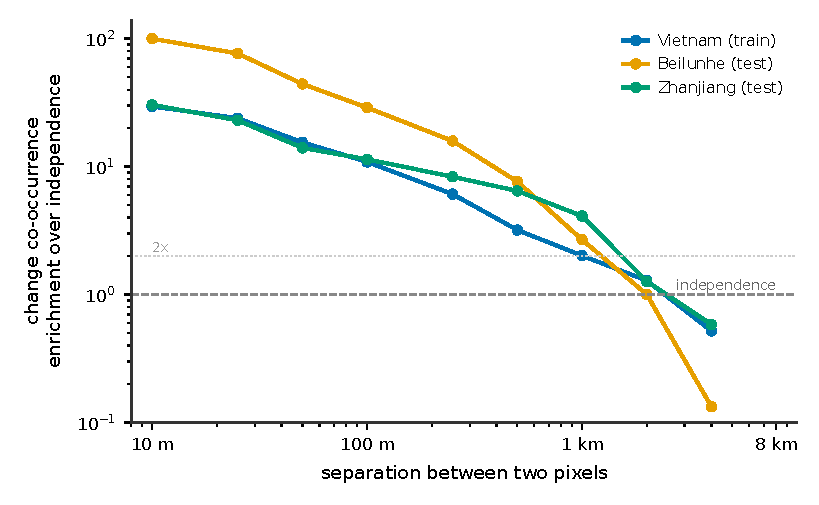
\includegraphics[width=\textwidth]{fig2_autocorr_decay.pdf}
\caption{Co-change enrichment $E(L) = C(L)/p^2$ as a function of pixel
separation $L$, computed on the full patch pools of all three regions
(Vietnam 76, Beilunhe 18, Zhanjiang 15 patches; change prevalence
$2.84\%$, $0.81\%$, $2.65\%$ respectively), averaged over the two
cardinal directions.
$E(L) = 1$ at independence; $E(L) > 1$ indicates positive spatial
autocorrelation of the change label. The curves fall below unity at the
largest lag (4\,km, beyond the 2\,km buffer); this sub-unity tail is not
interpreted as negative autocorrelation.}
\label{fig:autocorr}
\end{figure}

\subsection{Metrics and Spatial Inference}
\label{sec:eval}

Overall accuracy (OA), Cohen's kappa, mean intersection over union
(mIoU) and macro F1 over the four classes are reported, together with per-class producer's
and user's accuracy, IoU and F1. Because OA is dominated by the background
class, the $4\times4$ confusion matrix is additionally collapsed into a
$2\times2$ matrix (change = loss + gain vs.\ unchanged) and report $F1_{change}$, $IoU_{change}$, omission and commission. Overall accuracy has little discriminative power for this rare-event task (predicting ``no change'' everywhere already yields OA 0.974--0.992 at the three reference prevalences of 1.26\%, 0.81\% and 2.65\%) and is reported alongside the change metrics, never as the primary one; the change-class $F1$ and ROC-AUC are the co-primary metrics of this paper: $F1$ for comparability with the mangrove-mapping literature and thresholded operating-point diagnostics, ROC-AUC for prevalence-free discrimination. Cohen's kappa~\cite{foody2020kappa} is reported for comparability but, for the same reason, is not used for inference.

Every deep model was
trained with five random seeds (2026--2030); tables give mean
$\pm$ standard deviation over the five seeds, except for the pixel-level
baselines, which are deterministic given their sampled training pixels. It is
important to be precise about what that standard deviation is: the five seeds
re-draw the initialisation, the batch order and the augmentation stream on the
\emph{same} data and the \emph{same} split, so it measures optimisation
stochasticity only. It is not a dataset-level or spatial uncertainty and it does
not shrink with more seeds. The spatial uncertainty of any number in this paper
is bounded instead by the number of independent spatial units available
(2--5 per test region)---a quantity no amount of seed
repetition increases. All metrics are computed on the filtered patch subset
(mangrove fraction 5--85\%, Section~\ref{sec:split}) and are patch-weighted
(Section~\ref{sec:geom}). The per-architecture and per-split results are
summarised in Tables~\ref{tab:main} and~\ref{tab:rand}.

% ===== AUTO-GENERATED: paper tables — regenerate via `python3 analysis/make_latex_tables.py` (do not edit by hand) =====

\begin{table}[H]
\caption{Change-detection performance under the uniform (unweighted) class-weighting scheme, as mean $\pm$ std over seeds 2026--2030 (pixel-level baselines: single run). `Within' is the buffer-isolated held-out zone of the training region (Vietnam); Beilunhe and Zhanjiang are geographically disjoint test regions. $F1_{ch}$ / $IoU_{ch}$: binary change detection (loss + gain vs. unchanged) collapsed from the four-class output.}
\label{tab:main}
\centering
\footnotesize
\setlength{\tabcolsep}{3pt}
\resizebox{\textwidth}{!}{%
\begin{tabular}{llcccccc}
\toprule
 & & \multicolumn{3}{c}{Overall} & \multicolumn{2}{c}{Change class} \\
\cmidrule(lr){3-5}\cmidrule(lr){6-7}
Model & Region & OA & Kappa & mIoU & $F1_{ch}$ & $IoU_{ch}$ \\
\midrule
Random Forest (pixel) & Beilunhe & 0.943 & 0.705 & 0.437 & 0.180 & 0.099 \\
 & Zhanjiang & 0.944 & 0.524 & 0.369 & 0.016 & 0.008 \\
\addlinespace
SVM (RBF, pixel) & Beilunhe & 0.913 & 0.603 & 0.401 & 0.197 & 0.109 \\
 & Zhanjiang & 0.943 & 0.538 & 0.379 & 0.027 & 0.014 \\
\addlinespace
U-Net (Exp0) & within (Vietnam) & 0.941\,\scriptsize$\pm$0.019 & 0.741\,\scriptsize$\pm$0.065 & 0.451\,\scriptsize$\pm$0.028 & 0.270\,\scriptsize$\pm$0.018 & 0.156\,\scriptsize$\pm$0.012 \\
 & Beilunhe & 0.955\,\scriptsize$\pm$0.015 & 0.780\,\scriptsize$\pm$0.060 & 0.531\,\scriptsize$\pm$0.021 & 0.426\,\scriptsize$\pm$0.022 & 0.271\,\scriptsize$\pm$0.018 \\
 & Zhanjiang & 0.953\,\scriptsize$\pm$0.003 & 0.656\,\scriptsize$\pm$0.034 & 0.443\,\scriptsize$\pm$0.026 & 0.244\,\scriptsize$\pm$0.117 & 0.143\,\scriptsize$\pm$0.076 \\
\addlinespace
U-Net+CBAM (Exp1) & within (Vietnam) & 0.933\,\scriptsize$\pm$0.027 & 0.716\,\scriptsize$\pm$0.077 & 0.438\,\scriptsize$\pm$0.035 & 0.251\,\scriptsize$\pm$0.038 & 0.144\,\scriptsize$\pm$0.025 \\
 & Beilunhe & 0.948\,\scriptsize$\pm$0.017 & 0.752\,\scriptsize$\pm$0.062 & 0.507\,\scriptsize$\pm$0.030 & 0.369\,\scriptsize$\pm$0.166 & 0.236\,\scriptsize$\pm$0.111 \\
 & Zhanjiang & 0.953\,\scriptsize$\pm$0.004 & 0.649\,\scriptsize$\pm$0.062 & 0.445\,\scriptsize$\pm$0.037 & 0.277\,\scriptsize$\pm$0.158 & 0.168\,\scriptsize$\pm$0.099 \\
\addlinespace
DeepLabv3+ & within (Vietnam) & 0.946\,\scriptsize$\pm$0.017 & 0.760\,\scriptsize$\pm$0.057 & 0.455\,\scriptsize$\pm$0.022 & 0.273\,\scriptsize$\pm$0.009 & 0.158\,\scriptsize$\pm$0.006 \\
 & Beilunhe & 0.962\,\scriptsize$\pm$0.018 & 0.809\,\scriptsize$\pm$0.074 & 0.508\,\scriptsize$\pm$0.036 & 0.316\,\scriptsize$\pm$0.118 & 0.192\,\scriptsize$\pm$0.077 \\
 & Zhanjiang & 0.947\,\scriptsize$\pm$0.004 & 0.614\,\scriptsize$\pm$0.043 & 0.415\,\scriptsize$\pm$0.035 & 0.207\,\scriptsize$\pm$0.190 & 0.126\,\scriptsize$\pm$0.123 \\
\addlinespace
Temporal U-Net & within (Vietnam) & 0.952\,\scriptsize$\pm$0.014 & 0.772\,\scriptsize$\pm$0.052 & 0.459\,\scriptsize$\pm$0.022 & 0.242\,\scriptsize$\pm$0.002 & 0.138\,\scriptsize$\pm$0.002 \\
 & Beilunhe & 0.969\,\scriptsize$\pm$0.014 & 0.839\,\scriptsize$\pm$0.061 & 0.538\,\scriptsize$\pm$0.035 & 0.358\,\scriptsize$\pm$0.139 & 0.224\,\scriptsize$\pm$0.095 \\
 & Zhanjiang & 0.952\,\scriptsize$\pm$0.006 & 0.619\,\scriptsize$\pm$0.088 & 0.425\,\scriptsize$\pm$0.042 & 0.233\,\scriptsize$\pm$0.167 & 0.140\,\scriptsize$\pm$0.107 \\
\addlinespace
Temporal U-Net (GroupNorm) & within (Vietnam) & 0.958\,\scriptsize$\pm$0.003 & 0.793\,\scriptsize$\pm$0.012 & 0.451\,\scriptsize$\pm$0.028 & 0.153\,\scriptsize$\pm$0.141 & 0.088\,\scriptsize$\pm$0.081 \\
 & Beilunhe & 0.969\,\scriptsize$\pm$0.009 & 0.834\,\scriptsize$\pm$0.036 & 0.484\,\scriptsize$\pm$0.043 & 0.171\,\scriptsize$\pm$0.208 & 0.106\,\scriptsize$\pm$0.133 \\
 & Zhanjiang & 0.953\,\scriptsize$\pm$0.001 & 0.638\,\scriptsize$\pm$0.021 & 0.414\,\scriptsize$\pm$0.028 & 0.102\,\scriptsize$\pm$0.137 & 0.058\,\scriptsize$\pm$0.079 \\
\addlinespace
FC-Siam (SOTA baseline) & within (Vietnam) & 0.942\,\scriptsize$\pm$0.018 & 0.743\,\scriptsize$\pm$0.065 & 0.463\,\scriptsize$\pm$0.034 & 0.246\,\scriptsize$\pm$0.065 & 0.141\,\scriptsize$\pm$0.040 \\
 & Beilunhe & 0.949\,\scriptsize$\pm$0.026 & 0.760\,\scriptsize$\pm$0.104 & 0.514\,\scriptsize$\pm$0.061 & 0.381\,\scriptsize$\pm$0.144 & 0.243\,\scriptsize$\pm$0.102 \\
 & Zhanjiang & 0.949\,\scriptsize$\pm$0.009 & 0.658\,\scriptsize$\pm$0.055 & 0.455\,\scriptsize$\pm$0.036 & 0.423\,\scriptsize$\pm$0.049 & 0.269\,\scriptsize$\pm$0.039 \\
\addlinespace
ChangeFormer-style (Transformer) & within (Vietnam) & 0.836\,\scriptsize$\pm$0.047 & 0.373\,\scriptsize$\pm$0.143 & 0.282\,\scriptsize$\pm$0.047 & 0.019\,\scriptsize$\pm$0.024 & 0.010\,\scriptsize$\pm$0.013 \\
 & Beilunhe & 0.867\,\scriptsize$\pm$0.055 & 0.429\,\scriptsize$\pm$0.177 & 0.299\,\scriptsize$\pm$0.057 & 0.013\,\scriptsize$\pm$0.016 & 0.007\,\scriptsize$\pm$0.008 \\
 & Zhanjiang & 0.889\,\scriptsize$\pm$0.046 & 0.100\,\scriptsize$\pm$0.088 & 0.245\,\scriptsize$\pm$0.026 & 0.014\,\scriptsize$\pm$0.016 & 0.007\,\scriptsize$\pm$0.008 \\
\addlinespace
DeepLabv3+ (ImageNet-pretrained) & within (Vietnam) & 0.918\,\scriptsize$\pm$0.037 & 0.674\,\scriptsize$\pm$0.097 & 0.419\,\scriptsize$\pm$0.036 & 0.252\,\scriptsize$\pm$0.010 & 0.144\,\scriptsize$\pm$0.007 \\
 & Beilunhe & 0.946\,\scriptsize$\pm$0.024 & 0.742\,\scriptsize$\pm$0.084 & 0.453\,\scriptsize$\pm$0.058 & 0.224\,\scriptsize$\pm$0.117 & 0.130\,\scriptsize$\pm$0.072 \\
 & Zhanjiang & 0.946\,\scriptsize$\pm$0.003 & 0.579\,\scriptsize$\pm$0.021 & 0.388\,\scriptsize$\pm$0.015 & 0.080\,\scriptsize$\pm$0.062 & 0.042\,\scriptsize$\pm$0.035 \\
\addlinespace
U-Net+CBAM+MSA (Exp2) & within (Vietnam) & 0.941\,\scriptsize$\pm$0.009 & 0.737\,\scriptsize$\pm$0.031 & 0.448\,\scriptsize$\pm$0.015 & 0.253\,\scriptsize$\pm$0.043 & 0.146\,\scriptsize$\pm$0.028 \\
 & Beilunhe & 0.956\,\scriptsize$\pm$0.008 & 0.779\,\scriptsize$\pm$0.032 & 0.513\,\scriptsize$\pm$0.040 & 0.358\,\scriptsize$\pm$0.127 & 0.223\,\scriptsize$\pm$0.087 \\
 & Zhanjiang & 0.948\,\scriptsize$\pm$0.004 & 0.577\,\scriptsize$\pm$0.069 & 0.403\,\scriptsize$\pm$0.026 & 0.109\,\scriptsize$\pm$0.069 & 0.059\,\scriptsize$\pm$0.038 \\
\addlinespace
\bottomrule
\end{tabular}}
\end{table}



\begin{table}[H]
\caption{Spatial-autocorrelation control (Vietnam), primary uniform protocol. The same 60 non-buffer patches are re-assigned to a spatially interleaved random split (40/10/10) and re-trained and re-evaluated under an identical recipe, so the `honest' (buffer-isolated) and `leaky' (interleaved) arms differ in the spatial assignment of patches (a joint train--test reassignment; Section~\ref{sec:rand}). Pooled over 3 split draws $\times$ 3 run seeds, with collapsed runs excluded (see table note). $F1_{ch}$ / $IoU_{ch}$: binary change (loss + gain vs.\ unchanged); mean $\pm$ std over runs.}
\label{tab:rand}
{\footnotesize
\setlength{\tabcolsep}{3pt}
\begin{tabular}{llrrrrrc}
\toprule
Model & Protocol & OA & mIoU & $F1_{ch}$ & $IoU_{ch}$ & Comm. & Gap (pp) \\
\midrule
U-Net & honest & 0.969\,\scriptsize$\pm$0.000 & 0.497\,\scriptsize$\pm$0.002 & 0.284\,\scriptsize$\pm$0.007 & 0.165\,\scriptsize$\pm$0.005 & 0.482\,\scriptsize$\pm$0.015 &  \\
 & leaky & 0.962\,\scriptsize$\pm$0.001 & 0.654\,\scriptsize$\pm$0.028 & 0.603\,\scriptsize$\pm$0.038 & 0.433\,\scriptsize$\pm$0.040 & 0.263\,\scriptsize$\pm$0.023 & ${(+32.0)}$ \\
\addlinespace
U-Net+CBAM & honest & 0.969\,\scriptsize$\pm$0.001 & 0.496\,\scriptsize$\pm$0.002 & 0.282\,\scriptsize$\pm$0.011 & 0.164\,\scriptsize$\pm$0.007 & 0.487\,\scriptsize$\pm$0.021 &  \\
 & leaky & 0.963\,\scriptsize$\pm$0.002 & 0.654\,\scriptsize$\pm$0.027 & 0.601\,\scriptsize$\pm$0.036 & 0.431\,\scriptsize$\pm$0.037 & 0.271\,\scriptsize$\pm$0.026 & ${(+31.9)}$ \\
\addlinespace
U-Net+MSA & honest & 0.969\,\scriptsize$\pm$0.001 & 0.497\,\scriptsize$\pm$0.003 & 0.285\,\scriptsize$\pm$0.014 & 0.166\,\scriptsize$\pm$0.009 & 0.497\,\scriptsize$\pm$0.029 &  \\
 & leaky & 0.962\,\scriptsize$\pm$0.002 & 0.651\,\scriptsize$\pm$0.025 & 0.596\,\scriptsize$\pm$0.037 & 0.426\,\scriptsize$\pm$0.038 & 0.264\,\scriptsize$\pm$0.028 & ${(+31.2)}$ \\
\addlinespace
U-Net+CBAM+MSA & honest & 0.969\,\scriptsize$\pm$0.001 & 0.495\,\scriptsize$\pm$0.007 & 0.280\,\scriptsize$\pm$0.029 & 0.163\,\scriptsize$\pm$0.019 & 0.492\,\scriptsize$\pm$0.023 &  \\
 & leaky & 0.962\,\scriptsize$\pm$0.004 & 0.639\,\scriptsize$\pm$0.051 & 0.572\,\scriptsize$\pm$0.101 & 0.407\,\scriptsize$\pm$0.089 & 0.275\,\scriptsize$\pm$0.043 & ${(+29.3)}$ \\
\addlinespace
DeepLabv3+ & honest & 0.967\,\scriptsize$\pm$0.001 & 0.488\,\scriptsize$\pm$0.003 & 0.267\,\scriptsize$\pm$0.013 & 0.154\,\scriptsize$\pm$0.009 & 0.494\,\scriptsize$\pm$0.043 &  \\
 & leaky & 0.960\,\scriptsize$\pm$0.002 & 0.639\,\scriptsize$\pm$0.030 & 0.584\,\scriptsize$\pm$0.041 & 0.414\,\scriptsize$\pm$0.042 & 0.305\,\scriptsize$\pm$0.029 & ${(+31.7)}$ \\
\addlinespace
DeepLabv3+ (ImageNet-pretrained) & honest & 0.967\,\scriptsize$\pm$0.001 & 0.486\,\scriptsize$\pm$0.003 & 0.251\,\scriptsize$\pm$0.015 & 0.144\,\scriptsize$\pm$0.009 & 0.491\,\scriptsize$\pm$0.031 &  \\
 & leaky & 0.960\,\scriptsize$\pm$0.002 & 0.639\,\scriptsize$\pm$0.028 & 0.579\,\scriptsize$\pm$0.043 & 0.409\,\scriptsize$\pm$0.043 & 0.298\,\scriptsize$\pm$0.032 & ${(+32.8)}$ \\
\addlinespace
Temporal U-Net & honest & 0.968\,\scriptsize$\pm$0.001 & 0.495\,\scriptsize$\pm$0.004 & 0.293\,\scriptsize$\pm$0.012 & 0.172\,\scriptsize$\pm$0.008 & 0.530\,\scriptsize$\pm$0.024 &  \\
 & leaky & 0.959\,\scriptsize$\pm$0.002 & 0.643\,\scriptsize$\pm$0.030 & 0.590\,\scriptsize$\pm$0.038 & 0.420\,\scriptsize$\pm$0.038 & 0.319\,\scriptsize$\pm$0.045 & ${(+29.7)}$ \\
\addlinespace
Temporal U-Net (GroupNorm) & honest & 0.969\,\scriptsize$\pm$0.001 & 0.500\,\scriptsize$\pm$0.004 & 0.290\,\scriptsize$\pm$0.008 & 0.169\,\scriptsize$\pm$0.005 & 0.493\,\scriptsize$\pm$0.013 &  \\
 & leaky & 0.960\,\scriptsize$\pm$0.001 & 0.640\,\scriptsize$\pm$0.030 & 0.578\,\scriptsize$\pm$0.044 & 0.408\,\scriptsize$\pm$0.044 & 0.289\,\scriptsize$\pm$0.067 & ${(+28.8)}$ \\
\addlinespace
FC-Siam & honest & 0.965\,\scriptsize$\pm$0.006 & 0.491\,\scriptsize$\pm$0.013 & 0.289\,\scriptsize$\pm$0.014 & 0.169\,\scriptsize$\pm$0.010 & 0.512\,\scriptsize$\pm$0.034 &  \\
 & leaky & 0.956\,\scriptsize$\pm$0.004 & 0.627\,\scriptsize$\pm$0.020 & 0.562\,\scriptsize$\pm$0.034 & 0.392\,\scriptsize$\pm$0.033 & 0.283\,\scriptsize$\pm$0.024 & ${(+27.3)}$ \\
\addlinespace
ChangeFormer-style & honest & 0.966\,\scriptsize$\pm$0.001 & 0.471\,\scriptsize$\pm$0.006 & 0.196\,\scriptsize$\pm$0.020 & 0.109\,\scriptsize$\pm$0.013 & 0.387\,\scriptsize$\pm$0.029 &  \\
 & leaky & 0.952\,\scriptsize$\pm$0.003 & 0.493\,\scriptsize$\pm$0.009 & 0.314\,\scriptsize$\pm$0.068 & 0.188\,\scriptsize$\pm$0.050 & 0.292\,\scriptsize$\pm$0.056 & ${(+11.8)}$ \\
\addlinespace
\bottomrule
\end{tabular}
}
{\footnotesize Both arms of the contrast exclude runs that collapsed to an all- or near-all-background solution ($F1_{ch}<0.05$; 9 runs, ChangeFormer-style, Temporal U-Net (GN), U-Net, U-Net+CBAM, U-Net+CBAM+MSA), removed symmetrically when the sweep results were written; the affected families are unstable under the class imbalance rather than mis-measured, and retaining them in one arm only would bias the gap (Section~\ref{sec:rand}).}
\end{table}
% ===== END AUTO-GENERATED: paper tables =====

\section{Results}
\label{sec:results}

 Stated plainly: the same ten models, trained under an identical recipe, score
$26.9$--$34.1$ percentage points higher change $F1$ when test patches
interleave the training footprints than when a buffer separates them,
while their change-pixel ranking (ROC-AUC) differs by only $1.9$\,pp; the
gap is dominated by an operating-point (recall) shift rather than by the
rarity of change itself. Each subsection
follows one registered experiment (Appendix~\ref{app:reg}) and reports its result.

\subsection{The Spatial-Split Effect on the Score}
\label{sec:rand}

Same data, same architecture, same optimizer, same labels;
the only difference is the spatial split assignment---which patches go into
training and which go into testing. Both arms use three run seeds and draw
from the same pool of $60$ eligible patches (the $76$ Vietnam patches minus
the $16$ within the ${\geq}2$\,km buffer), with the same $40/10/10$
 train/validation/test sizes and recipe. The isolated arm uses a fixed
buffer-separated zone assignment (the same $40$ training patches and the same
$10$ test patches for every draw); the interleaved arm re-partitions the full
pool randomly for each draw, so its training, validation, and test composition
all shift with the draw; in this arm, 85\% of test patches are adjacent to
or overlap a validation patch (55/100 have footprint overlap; median minimum
edge-to-edge distance $0$\,km), so validation-based early stopping is spatially
proximate to the test set. Because the interleaved arm draws its training,
validation, and test patches from the same pool, this val--test proximity is a
component of the interleaved protocol by construction rather than an independent
confound; it is part of what the interleaved protocol measures, and the
checkpoint-selection channel it opens is bounded below (Section~\ref{sec:limitations}).
The isolated arm's slight variation across the ten
partitions ($0.268$--$0.281$) reflects the different seed triplets drawn from
the five-seed primary sweep ($C(5,3){=}10$), not a change in data composition.
Under a spatially interleaved random assignment, change-class $F1$ is
$29.6$ percentage points higher than under a buffer-separated assignment when
the 81 non-collapsed runs are pooled ($26.9$--$34.1$\,pp across the three
split draws, Table~\ref{tab:split}), and every architecture gains: $+11.8$ to
$+32.8$\,pp at the model-mean level. Because the interleaved arm re-partitions
the pool, $6$--$10$ of its $10$ test patches were training or validation
under the isolated assignment---the contrast is not a pure test-side
substitution but a joint train--test reassignment
(Section~\ref{sec:prevalence} quantifies the test-side component).
 Nine of the 90 runs reach a near-zero change $F1$ under the uniform-weighting recipe
and are excluded under a pre-specified validity filter ($F1_{ch}<0.05$):
four U-Net-family runs (split $k{=}3$, seed 2026) and five ChangeFormer runs
(spread across splits and seeds). The same nine also fall below the threshold
on the honest arm, so the filter is symmetric: the collapsed runs are
identified by model and split/seed, not by arm, and the same model/split/seed
combination collapses in both arms. Because both arms are read from the same
sweep, the filter cannot favour either one, and the contrast does not depend
on it: re-admitting all
90 runs symmetrically gives a pooled gap of $+26.7$\,pp (per-run range
$+0$ to $+39$\,pp) instead of $+29.6$\,pp on the 81 retained runs, with every
conclusion of this section unchanged. The per-architecture range widens to
$+5.3$ to $+32.8$\,pp because ChangeFormer-style, whose interleaved arm is the
weakest in the suite ($F1_{ch}=0.314$ against $0.56$--$0.60$ for the other
nine architectures), gains the least from interleaving.
What changed is the evaluation protocol---the training distribution, the test
composition, and the spatial configuration all shift simultaneously.


This is not an architecture effect. The phenomenon is consistent in
direction across all ten deep architectures,
but this consistency is secondary evidence: the ten architectures share the
same training data, the same split, and the same recipe, so their directional
agreement is primarily driven by the shared protocol effect, not by independent
replication. No architecture ranking is performed: the suite's batch size, input
representation, initialisation, and weight sharing are confounded with
architecture, and the per-model point estimates rest on $2$--$5$ spatial units.
The primary evidence is the pooled split-level contrast; the per-model
consistency is a sanity check, not a replication
(Figure~\ref{fig:rand}).

\begin{figure}[H]
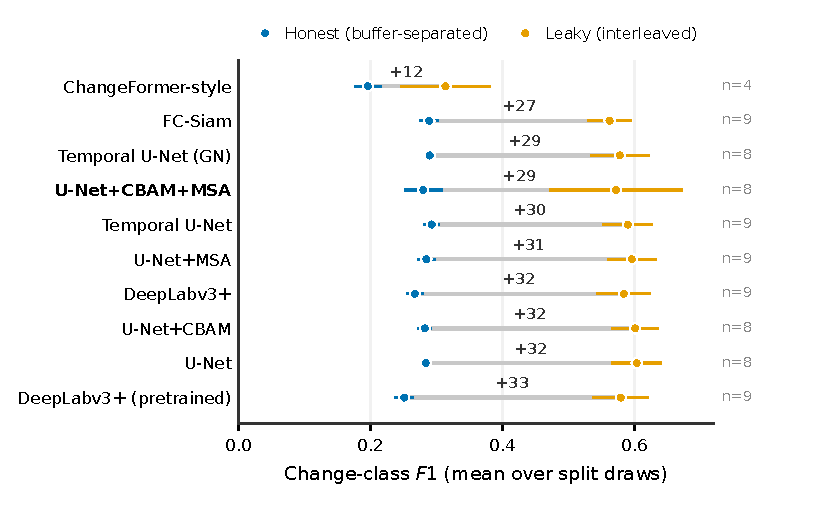
\includegraphics[width=\textwidth]{fig3_per_arch_gap.pdf}
\caption{Per-architecture change-$F1$ under the honest (buffer-separated) and
leaky (interleaved) protocols, uniform weighting. Both arms draw from the
same $60$-patch pool and share recipe and run seeds; the isolated arm uses a
fixed zone assignment while the interleaved arm re-partitions the pool per
draw. Each row joins the honest mean (blue) to the leaky mean
(amber); the label on the connector is the inflation in percentage points and
rows are ordered by it, with the right-hand column giving the number of split
draws contributing to each mean. Error bars are the standard deviation over
those pooled runs (eight to nine per architecture, four for
ChangeFormer-style).}
\label{fig:rand}
\end{figure}

\begin{table}[H]
\centering
 \caption{Per-split $F1_{\text{change}}$ gap (pooled over all ten models),
uniform weighting.
Each split draw $k$ randomly assigns the 60 eligible patches
(76 total $-$ 16 within the ${\geq}2$\,km buffer) to a 40/10/10
train/val/test split for the leaky arm; the honest arm keeps the fixed
buffer-separated assignment. The honest arm's slight variation
($0.280$/$0.279$/$0.268$) reflects the different seed triplets per draw
($C(5,3){=}10$ partitions), not a change in data composition.}
\label{tab:split}
\begin{tabular}{lccc}
\toprule
Split draw & Honest & Leaky & Gap (pp) \\
\midrule
$k{=}1$ & $0.280$ & $0.548$ & $+26.9$ \\
$k{=}2$ & $0.279$ & $0.620$ & $+34.1$ \\
$k{=}3$ & $0.268$ & $0.544$ & $+27.6$ \\
\midrule
Pooled & $0.276$ & $0.572$ & $+29.6$ \\
\bottomrule
\end{tabular}
\end{table}

Because the headline rests on
three split draws, the entire counterfactual was repeated on ten independently
drawn partitions of the same eligible patch pool (ten architectures $\times$
three run seeds, 300 runs; 270 non-collapsed, the same $30$ collapses as a
proportion as the three-draw set, Table~\ref{tab:partitions}). The gap is
positive in all ten partitions (per-partition means $+24.3$ to $+35.4$\,pp,
pooled $+29.6$\,pp), giving a partition-level 95\% interval of $+26.9$ to
$+32.2$\,pp (t-based on the ten partition means; cluster $=$ partition). The pooled value is unchanged from the
three-draw headline. The interval is narrow, but it does not by itself rule out
a region-specific effect: these ten partitions are independent random draws yet
strongly correlated---the region holds only $\sim\!60$ eligible patches and any
two partitions share $57.5$--$75\%$ of their 40 training patches---so it bounds
partition-sampling variability within this one region, not replication across
ten spatially disjoint regions.

\begin{table}[H]
\centering
\caption{The spatial-interleaving gap across ten independently drawn
partitions, uniform weighting, pooled over all ten models per partition
(collapse-excluded). Each partition randomly assigns the same 60 eligible
patches to a 40/10/10 train/val/test split; the honest arm keeps the
buffer-separated assignment. Positive in $10/10$ partitions; pooled
$+29.6$\,pp, partition-level 95\% interval $+26.9$ to $+32.2$\,pp.}
\label{tab:partitions}
\begin{tabular}{ccccc}
\toprule
Partition & Honest & Leaky & Gap (pp) & $n$ (non-collapsed) \\
\midrule
$k{=}1$ & $0.280$ & $0.548$ & $+26.9$ & 28 \\
$k{=}2$ & $0.279$ & $0.620$ & $+34.1$ & 28 \\
$k{=}3$ & $0.268$ & $0.544$ & $+27.6$ & 25 \\
$k{=}4$ & $0.281$ & $0.553$ & $+27.1$ & 26 \\
$k{=}5$ & $0.276$ & $0.553$ & $+27.7$ & 27 \\
$k{=}6$ & $0.274$ & $0.586$ & $+31.2$ & 27 \\
$k{=}7$ & $0.271$ & $0.550$ & $+28.0$ & 28 \\
$k{=}8$ & $0.279$ & $0.612$ & $+33.3$ & 28 \\
$k{=}9$ & $0.275$ & $0.628$ & $+35.4$ & 26 \\
$k{=}10$ & $0.277$ & $0.519$ & $+24.3$ & 27 \\
\midrule
Pooled & $0.276$ & $0.572$ & $+29.6$ & 270 \\
\bottomrule
\end{tabular}
\end{table}

The gap is a gain-class effect. Splitting the pooled change-$F1$
into its two change classes (Table~\ref{tab:lossgain}), the per-class gap is
larger for the \emph{gain} class (new mangrove) than for the \emph{loss} class
(lost mangrove): the gain class moves from $F1\approx0.008$ under the
buffer-separated assignment to $0.609$ under the interleaved one
($+60.2$\,pp), whereas loss moves from $0.345$ to $0.528$ ($+18.3$\,pp). Under
the disjoint protocol the models therefore recover essentially none of the new
mangrove, and the change-$F1$ inflation is carried disproportionately by that
single rare, spatially discontinuous class rather than by the two classes in
proportion to their support.

\begin{table}[H]
\centering
\caption{Per-class change-$F1$ under the honest (buffer-separated) and leaky
(interleaved) protocols, uniform weighting, pooled over the same 81
non-collapsed runs as Table~\ref{tab:split}. The per-class gap is larger for
the gain (new mangrove) class than for the loss (lost mangrove) class.}
\label{tab:lossgain}
\begin{tabular}{lccc}
\toprule
Change class & Honest & Leaky & Gap (pp) \\
\midrule
loss (mangrove lost) & $0.345$ & $0.528$ & $+18.3$ \\
gain (mangrove new) & $0.008$ & $0.609$ & $+60.2$ \\
\bottomrule
\end{tabular}
\end{table}

\subsection{The $F1$ Gap versus ROC-AUC Discrimination}
\label{sec:metric}

The same
90 runs that differ by $+29.6$\,pp in change $F1$ (pooled over the 81
non-collapsed runs; the nine collapsed runs are excluded from $F1$---seven
predict no change pixels at all, and the other two predict a few, with
precision $\geq 0.79$ but recall $\leq 0.02$) differ by only $+1.9$\,pp in
ROC-AUC (computed on all 90 runs, since the metric is defined even at zero
positive predictions) and $+12.5$\,pp in balanced
accuracy at $0.5$ (prevalence-free, threshold-fixed;
Table~\ref{tab:metrics}). The evaluation protocol changes not only which
examples are tested but also how the predictions are converted into a score:
$F1$ is thresholded, prevalence-sensitive, and argmax-dependent, while ROC-AUC
is a ranking measure (the binary change score for ranking is the summed
softmax probability of the loss and gain classes). The $+12.5$\,pp BA gap is intermediate between the two: at a fixed $0.5$
threshold the models trained on the interleaved split have different operating
characteristics on the two test sets, so BA moves less than $F1$ (which is
additionally prevalence-sensitive) but far more than ROC-AUC (which integrates
over all thresholds). Nine of 90 runs (7 with $F1$ exactly zero, 2 near-zero) score near-zero
change $F1$ while ranking change pixels at ROC-AUC $0.77$--$0.97$, because
their change probability never becomes a per-pixel maximum and the hard
decision rule therefore fires on few or no pixels. A model can rank change
pixels well and still receive a near-zero $F1$; this is a property of the
metric under extreme imbalance, not of the model
(Figure~\ref{fig:collapse}).

\begin{figure}[H]
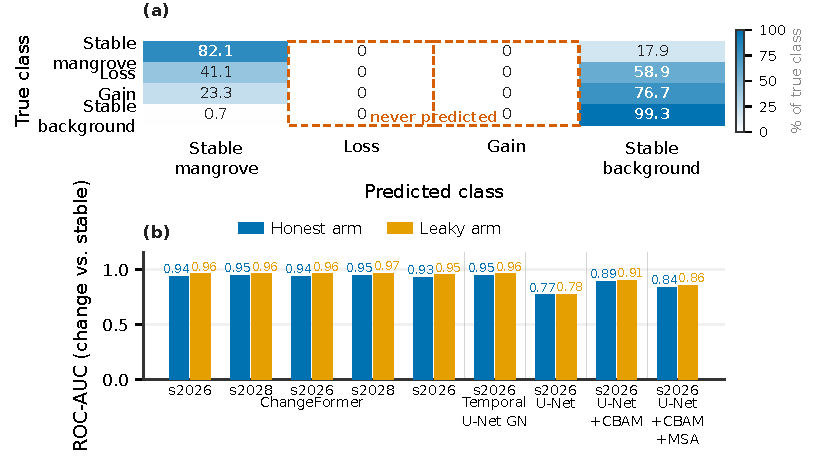
\includegraphics[width=\textwidth]{fig4_collapse.pdf}
\caption{Hard-decision failure vs.\ soft-probability ranking in collapsed
runs.
(a) Representative confusion matrix (ChangeFormer, seed 2026, leaky
arm) showing zero change predictions; the dashed box marks the Loss and Gain
columns, which are never predicted at all.
(b) ROC-AUC for all 9 collapsed runs, honest (blue) vs.\ leaky
(amber), range $0.77$--$0.97$;
the models rank change well in probability space but the change
probability rarely becomes the per-pixel argmax under extreme class
imbalance (prevalence $1.3\% \to 2.9$--$3.8\%$), yielding
$F1_{\text{change}}$ below the 0.05 validity threshold in all 9 runs:
exactly zero in seven, and in the remaining two the few predicted change
pixels carry precision $\geq 0.79$ but recall $\leq 0.02$.}
\label{fig:collapse}
\end{figure}

% ===== AUTO-GENERATED by analysis/roc_auc_prevalence.py -- do not edit =====
\begin{table}[H]
\centering
\small
\caption{The same 90 paired runs scored under four metrics of increasing
prevalence sensitivity. The interleaved test set carries
$2.68\times$ the change prevalence of the isolated one.
$n{=}81$ for F1-based metrics (nine collapsed runs excluded); $n{=}90$
for ROC-AUC and balanced accuracy.
Per-model: range of ten architecture means; Run range: over 90 paired runs.}
\label{tab:metrics}
\setlength{\tabcolsep}{3.5pt}
\begin{tabular}{lrrrl}
\toprule
Metric & Mean gap (pp) & Run range & Per-model & Sensitive to \\
\midrule
ROC-AUC & $+1.9$ & $[-0.5$, $+3.6$] & $+0.9$, $+2.3$ & neither \\
Bal. accuracy (0.5) & $+12.5$ & $[0.0$, $+20.4]$ & $+1.5$, $+15.6$ & threshold \\
MCC (0.5) & $+23.9$ & $[-1.0$, $+34.0$] & $+4.3$, $+28.6$ & both \\
AP / PR-AUC & $+33.7$ & $[+6.5$, $+42.4$] & $+29.9$, $+36.6$ & both \\
\bottomrule
\end{tabular}
\end{table}
%% ===== END AUTO-GENERATED (metric comparison) =====

To isolate the prevalence contribution, each leaky-run AP is recomputed at
the honest-run prevalence by evaluating the precision--recall curve at the
target prevalence (exact method; the first-order rescaling
$\mathrm{AP}_{\text{leaky}}\times\bar{\pi}_{\text{h}}/\pi_{\text{l}}$
underestimates the corrected AP in this $\pi$ range).
After this correction the mean AP gap is $+15.2$\,pp (range $-0.5$ to
$+23.9$, positive in 52 of 54 runs\footnote{The 54-run subset comprises the
six architectures with available checkpoints; the other four enter the
uncorrected 90-run statistic (Table~\ref{tab:split}).},
Table~\ref{tab:split}). The split is made within this same subset, whose
uncorrected AP gap is $+32.9$\,pp (range $+6.5$ to $+42.4$): the prevalence
correction removes $17.7$\,pp, about half, leaving a
high-precision-region ranking advantage of $+15.2$\,pp. (The full
ten-architecture, 90-run sweep of Table~\ref{tab:split} gives the uncorrected
$+33.7$\,pp headline quoted elsewhere.) A ROC-AUC gap of $+1.9$\,pp is
consistent with a small global-ranking shift concentrated in the low-FPR
region (Figure~\ref{fig:rocpr}).

\begin{figure}[H]
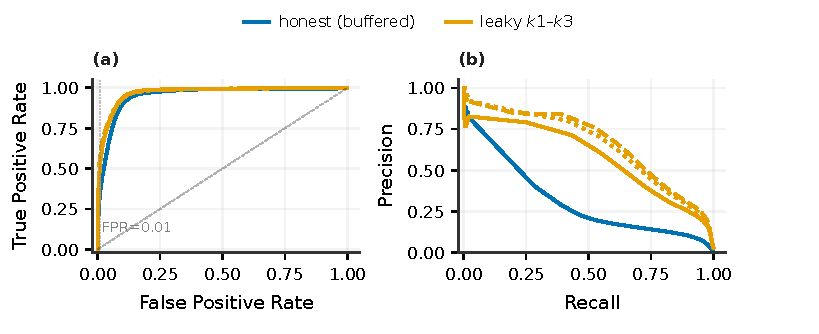
\includegraphics[width=\textwidth]{fig5_roc_pr.pdf}
\caption{ROC and precision--recall curves for a representative model
(U-Net+CBAM+MSA, seed 2027) on the Vietnam test set.
(a) ROC curves; (b) precision--recall curves.
Blue: honest (separated) test set ($\pi=1.3\%$).
Orange: interleaved (leaky) test draws k1--k3 ($\pi=2.9$--$3.8\%$), drawn solid,
dashed and dotted respectively.
Dashed grey line: FPR~$=$~0.01 operating threshold.
ROC-AUC is prevalence-free, $F1$ is not.}
\label{fig:rocpr}
\end{figure}

The gap is also an operating-point effect.
Holding the model fixed (one checkpoint, scored once) and varying only the test
set and the decision rule, the change-$F1$ gap is $+29.7$\,pp at the
argmax point (the single-checkpoint value; the 81-run pooled headline is
$+29.6$\,pp) but only $+8.1$\,pp when a single threshold, chosen on the shared
held-out validation set, is applied to both arms
(Table~\ref{tab:operating}). Scoring each arm at its own $F1$-maximising
threshold (oracle) or pinning both arms to $\mathrm{FPR}=1\%$ leaves the gap
essentially unchanged ($+28.6$\,pp), so it is not a pure hard-decision or
single-threshold artefact. The contrast between the per-arm points
($+25$--$29$\,pp) and the shared-threshold point ($+8.1$\,pp) is the
interleaved arm's lower, prevalence-matched operating threshold: because its
test set carries $\sim2.7\times$ the change prevalence, its $F1$-optimal
threshold is lower, and cutting there harvests a denser band of true change
pixels that a shared threshold, matched to the lower-prevalence arm, does not.
A residual of $+8.1$\,pp survives even under this fair shared-threshold
protocol, the prevalence arithmetic that remains at a common operating point.

\begin{table}[H]
\centering
\caption{Change-$F1$ gap (interleaved minus honest) as the operating threshold
varies, with training held fixed (k1 draw) and the ten architectures pooled.
Per-arm points (argmax, FPR-pinned, oracle) let each arm use its own threshold;
the validation point applies one shared threshold chosen on the held-out
validation set.}
\label{tab:operating}
\begin{tabular}{lcc}
\toprule
Operating point & Threshold policy & Gap (pp) \\
\midrule
argmax (four-class) & per-arm & $+29.7$ \\
FPR $=1\%$ (pinned) & per-arm & $+28.6$ \\
FPR $=5\%$ (pinned) & per-arm & $+25.4$ \\
oracle ($F1$-maximising) & per-arm & $+28.6$ \\
shared validation threshold & one for both & $+8.1$ \\
\bottomrule
\end{tabular}
\end{table}

\subsection{Decomposing the Gap Between Prevalence Arithmetic and the Recall Shift}
\label{sec:prevalence}

\emph{This section decomposes the $+29.6$\,pp gap in three steps: a $2\times2$
 factorial that separates the training-side, test-side and joint components;
and a direct
prevalence reweighting that measures the case-mix term on its own.}

\emph{A $2\times2$ train/test spatial factorial (E2).} The counterfactual above
compares two corners of the design; it is completed with I/R---the \emph{same}
training zone (40 patches) and the \emph{same} validation zone as the I/I main
sweep, but a random test set of 10 patches drawn (fixed RNG seed) from the 26
non-train, non-validation patches, so test patches interleave with the training
zone (edge distances $0$--$12.8$\,km). The four cells are reported in
Table~\ref{tab:factorial}. Three independent random draws $\times$
five run seeds $\times$ five models were trained for I/R; the R/I and R/R cells
pool the 3-split-seed $\times$ 3-run-seed sweep, and I/I is the within-region
result of the primary five-seed sweep. With
$\Delta_{\mathrm{train}} = \mathrm{RI}-\mathrm{II}$,
$\Delta_{\mathrm{test}} = \mathrm{IR}-\mathrm{II}$ and
$\Delta_{\mathrm{int}} = \mathrm{RR}-\mathrm{RI}-\mathrm{IR}+\mathrm{II}$:

\begin{table}[H]
\centering
\caption{Spatial $2\times2$ train/test factorial, change-class $F1$ (within-region, uniform weighting).
I~$=$~isolated zone, R~$=$~interleaved random.
I/I: primary five-seed sweep (Table~\ref{tab:main}); R/I and R/R: 3 split $\times$ 3 run seeds;
I/R: 15 runs (3 test draws $\times$ 5 seeds).
Components (pp, pre-rounding): $\Delta_{\mathrm{train}}{=}\mathrm{RI}{-}\mathrm{II}$,
$\Delta_{\mathrm{test}}{=}\mathrm{IR}{-}\mathrm{II}$,
$\Delta_{\mathrm{int}}{=}\mathrm{RR}{-}\mathrm{RI}{-}\mathrm{IR}{+}\mathrm{II}$.}
\label{tab:factorial}
{\small
%% ===== AUTO-GENERATED by analysis/make_factorial_tables.py tab:factorial
%% ===== AUTO-GENERATED by analysis/make_factorial_tables.py tab:factorial
\begin{tabular}{l cccc ccc}
\toprule
 & \multicolumn{4}{c}{Cells (change $F1$)} & \multicolumn{3}{c}{Components (pp)} \\
Model & I/I & R/I & R/R & I/R & $\Delta_{\mathrm{train}}$ & $\Delta_{\mathrm{test}}$ & $\Delta_{\mathrm{int}}$ \\
\midrule
U-Net & 0.268 & 0.286 & 0.606 & 0.326 & $+1.8$ & $+5.8$ & $+26.1$ \\
U-Net+CBAM & 0.244 & 0.286 & 0.605 & 0.333 & $+4.2$ & $+9.0$ & $+22.9$ \\
U-Net+CBAM+MSA & 0.252 & 0.283 & 0.576 & 0.366 & $+3.2$ & $+11.4$ & $+17.8$ \\
DeepLabv3+ & 0.275 & 0.267 & 0.584 & 0.353 & $-0.8$ & $+7.8$ & $+23.9$ \\
Temporal U-Net & 0.241 & 0.293 & 0.590 & 0.335 & $+5.1$ & $+9.3$ & $+20.4$ \\
\bottomrule
\end{tabular}
%% ===== END AUTO-GENERATED (factorial tables) =====
%% ===== END AUTO-GENERATED (factorial tables) =====
}
\par\vspace{4pt}
{\footnotesize I/R run-to-run std (15 runs; 12 for U-Net+CBAM+MSA):
$0.024$--$0.055$.
Four U-Net-family collapsed runs are excluded from the factorial cells
(globally, nine of the 90 runs collapse: 4 U-Net family + 5 ChangeFormer);
including them lowers U-Net-family R/R by 0.06--0.07.
Confidence intervals for the three components are deferred to a follow-up:
the cells above are collapse-excluded summary statistics, and a per-run
resampling does not reproduce these exact point estimates, so a consistent
run-set re-derivation is required before CIs are reported.}
\end{table}

The decomposition is consistent across the five architectures
(Table~\ref{tab:factorial}): the composite test-side component
$\Delta_{\mathrm{test}} + \Delta_{\mathrm{int}} \approx +29$--$+32$\,pp
dominates, the training-side component $\Delta_{\mathrm{train}}$ spans
$-0.8$ to $+5.1$\,pp, and the I/R sweep splits the test-side component
into a modest test-assignment contrast $\Delta_{\mathrm{test}} = \mathrm{IR} -
\mathrm{II}$ ($+5.8$ to $+11.4$\,pp) and a large positive joint-assignment
interaction
$\Delta_{\mathrm{int}}$ ($+17.8$ to $+26.1$\,pp). The interaction has a direct
geometric explanation. The edge distance of every test patch to
the training zone of its own split was measured (512\,px patch footprints on the
256\,px grid, 2.56\,km per step; audit script listed in
Appendix~\ref{app:repro}): in the random/random protocol,
\emph{every} test patch lies at edge distance 0 from the (random) training
set (30/30 for the three primary splits, 100/100 for the ten secondary
splits), and 30/30 (primary) / 98/100 (secondary) overlap the footprint of
at least one training patch; in I/R, only 8 of the 30 draws (27\%;
3/2/3 per draw) touch the spatially separated training zone, the remaining
22 lying 2.56--12.8\,km away. Edge distance (gap between patch edges) and
footprint overlap (shared area) are distinct quantities: at a 256\,px
anchor difference the patches overlap by 256\,px with zero edge gap, and at
512\,px they touch without overlapping (zero edge gap); the
``edge distance 0'' counts both cases, and the overlap count is the
stricter subset (98/100). Randomising the test set therefore pays off only when
the training zone is also interleaved---train--test contact is set jointly
by the two assignments, which is what a positive interaction encodes here.
The pattern is therefore consistent with the inflation arising from joint
train--test proximity rather than from the training assignment alone, with a
training-side contribution that is near zero and not robust in sign.

The factorial bounds the effect but does not attribute it. The four cells differ in
more than the manipulated assignment: re-randomising the training (or test) set
simultaneously changes the train--test distance distribution, the footprint
overlap, the local
class prevalence and the spatial morphology of the sampled patches. Only the
case-mix difference is measured directly (next paragraph). The distance
distribution and the morphology are not held fixed in any cell, so
$\Delta_{\mathrm{train}}$, $\Delta_{\mathrm{test}}$ and
$\Delta_{\mathrm{int}}$ are \emph{design-factor contrasts of the spatial
arrangement} and nothing more. They are not read as causal attributions to the
training side, to the test side, or to overlap in particular; the
overlap-free control (Section~\ref{sec:e3}) does not reproduce
the headline at reduced scale, though it does not quantify what a fully powered
version would show.

The prevalence component is measurable, and it is small. The
factorial's $\Delta_{\mathrm{test}} = +5.8$--$+11.4$\,pp is sometimes read as a
pure prevalence (case-mix) effect, but this is incorrect: the I/R and I/I cells
share the \emph{same} interleaved training zone, so $\Delta_{\mathrm{test}}$
reflects differences in the test set's prevalence, spatial morphology, local
neighborhood, and patch composition jointly. To isolate the prevalence
arithmetic, a direct reweighting was performed: for each of the 81
non-collapsed runs (10 models $\times$ 3 splits $\times$ 3 seeds, minus 9
collapsed), the honest arm's TPR and FPR were extracted from the confusion
matrix under the four-class argmax decision (the same rule that produces
$F1_{\text{change}}$), then F1 was recomputed at that run's own interleaved
(leaky) prevalence --- $2.9\%$ to $3.8\%$ across the three split draws, mean
$3.37\%$ --- while holding its TPR and FPR constant. The prevalence-only
shift is $+2.7$\,pp on average (range $+0.8$ to $+3.4$\,pp across models;
$+0.8$ for ChangeFormer-style, $+3.4$ for Temporal U-Net).
The change-class $F1$ as a function of prevalence $\pi$, TPR, and FPR is:
\begin{equation}
F1(\pi,\,\text{TPR},\,\text{FPR})
= \frac{2\,\pi\,\text{TPR}}
{2\,\pi\,\text{TPR} + \pi - \pi\,\text{TPR} + (1-\pi)\,\text{FPR}}
= \frac{2\,\pi\,\text{TPR}}
{\pi + \pi\,\text{TPR} + (1-\pi)\,\text{FPR}}.
\label{eq:f1decomp}
\end{equation}
A full decomposition of the $F1$ gap is computed for each run, walking from
its honest $(\pi,\text{TPR},\text{FPR})$ triple to its own interleaved
(leaky) triple (mean prevalence $3.37\%$), and attributes the difference to
shifts in TPR, FPR, and $\pi$.
The decomposition is order-dependent because $F1$ is nonlinear in all
three arguments; the path reported is: prevalence first
(at the honest operating point, $+2.7$\,pp), then FPR ($-2.7$\,pp), then TPR
($+29.6$\,pp). The three terms sum to $+29.6$\,pp, matching the observed
$+29.6$\,pp mean gap exactly (81 non-collapsed runs), because a sequential
path through Equation~\ref{eq:f1decomp} telescopes. The TPR term dominates
under any ordering ($+25.4$ to $+31.6$\,pp); the prevalence term is $+2.7$ to
$+9.6$\,pp and the FPR term $-2.7$ to $-9.8$\,pp, so the attribution between
$\pi$ and the operating point is path-dependent while the total is not
(Figure~\ref{fig:decomp}).

\begin{figure}[H]
\centering
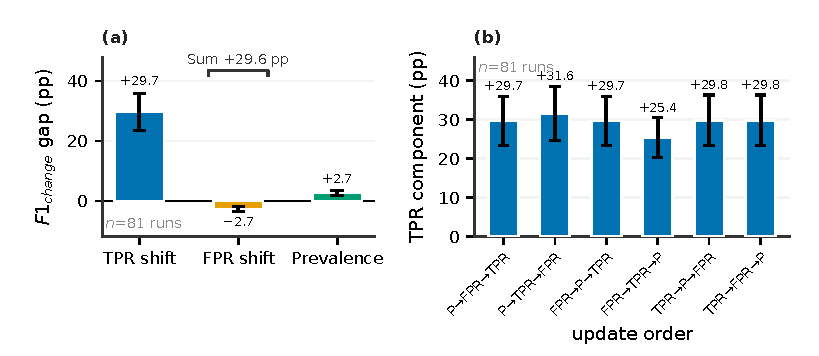
\includegraphics[width=\textwidth]{fig6_decomposition.pdf}
\caption{Decomposition of the $+29.6$\,pp $F1$ change gap
(ten-model pool, 81 non-collapsed runs) into TPR shift
($+29.6$\,pp), prevalence arithmetic ($+2.7$\,pp), and FPR shift
($-2.7$\,pp).
(a) Component means with 81-run standard deviations.
(b) TPR component under the six orderings in which prevalence, FPR and TPR are
updated (range $+25.4$ to $+31.6$\,pp), showing that the TPR shift is the
dominant driver regardless of decomposition order.
Honest arm: $\pi = 1.3\%$, FPR $= 0.2\%$; leaky arm: $\pi = 3.4\%$,
FPR $= 0.7\%$. Jensen residual (mean-of-runs minus run-of-means)
$0.4$\,pp.}
\label{fig:decomp}
\end{figure}

The dominant component is the TPR shift ($+29.6$\,pp). The ROC-AUC gap is
$+1.9$\,pp (honest $0.946$ vs.\ interleaved $0.965$, mean over 90 runs),
indicating that the overall ranking ability is similar, but the TPR
difference under the argmax decision (FPR $0.002$ vs.\ $0.007$) is concentrated
in the low-FPR operating region where $F1$ is computed. The factorial
decomposition (Table~\ref{tab:factorial}, Section~\ref{sec:prevalence})
clarifies the source: the full inflation ($+30.9$ to $+36.1$\,pp,
I/I $\to$ R/R) has the training$\times$test interaction as its
largest component, exceeding either main effect. The training-side term
changes sign across architectures---positive for U-Net and the U-Net+CBAM
family, negative for DeepLabv3+---so a simple training-distribution shift
does not account for the pattern. This is a
joint spatial configuration effect, not a simple calibration shift. The
FPR increase ($+0.5$\,pp) slightly reduces F1 via the precision
denominator. The balanced-accuracy gap of $+12.5$\,pp
(Table~\ref{tab:metrics}, all 90 runs) is consistent with this
decomposition. The $1.9$\,pp difference between the $+12.5$\,pp
(all-run mean) and the $+14.4$\,pp implied by the 81 non-collapsed
runs' mean TPR/FPR is due to the 9 collapsed runs (all- or
near-all-background predictions, BA gap $\approx 0$) diluting the all-run average.

Two reasons to read the factorial bounds as bounds rather than a decomposition.
The I/R cell's test-set prevalence ($1.70\%$) is itself above the honest
$1.26\%$, so $\Delta_{\mathrm{test}}$ includes a residual prevalence
component. And the remainder is labelled by the geometry it co-varies with,
not by a measurement: it is a joint proximity contrast, of which shared
 footprint is one component and residual kilometre-scale proximity another.
The I/R cell rests on three
independent random test arrangements (15 runs per model; 12 for
U-Net+CBAM+MSA after excluding the collapsed seed; run-to-run standard
deviation $0.024$--$0.055$), fewer than the three split arrangements behind
the R-side cells.

\subsection{The Dominant but Non-Decomposable Joint Spatial Configuration}
\label{sec:joint}

The dominant component of the gap---the $+29.6$\,pp TPR shift at the fixed
threshold---is associated with the joint spatial configuration of training and
test samples: a configuration that bundles footprint overlap, near-neighbor
proximity, and spatial morphology into a single factor. The $2\times2$
factorial separates a small prevalence-arithmetic shift ($+2.7$\,pp) from the
joint-proximity contrast but not overlap from proximity within the latter;
re-drawing a split changes distance, overlap, prevalence, and morphology at
once, so all factorial components are design-factor contrasts rather than
causal estimates (Section~\ref{sec:prevalence}). The geometric evidence does allow a
prior ranking of candidates: all $30$ of
$30$ overlapping test patches share pixels with training patches (footprint
overlap is ubiquitous at the $2.56$\,km grid snap); co-change enrichment decays
from $\sim$30$\times$ at $10$\,m to below unity by $1$--$2$\,km (kilometre-scale
proximity is bounded); and the morphological boundary effect is a one-pixel
displacement ($0.003$--$0.128$\,$F1$) that is flat beyond that. These make
footprint overlap and near-neighbour proximity the leading candidates among the
bundled factors; no claim is made that their individual
contributions have been identified.

\subsection{The E3 Overlap-Free Control}
\label{sec:e3}

E3-C applies the same control at a reduced patch geometry (128\,px pool).
E3-B (block-interleaved, 16 splits, 3 architectures) and E3-C (reduced 128\,px
geometry) are two variants of the overlap-free control. E3-B's reduced scale is
a consequence of one design choice, not a property of the
landscape: at $512$\,px on a $256$\,px stride the extracted patches overlap, so
a random assignment always shares pixels. Setting the step equal to the patch
size makes the pool disjoint, and a random assignment of a disjoint pool is
already overlap-free. The training region was rebuilt at $128$\,px with a
$128$\,px step, which leaves $155$ patches after the mangrove and clear-fraction
filters, and ran both arms at the full $40/10/10$ size
(Section~\ref{app:repro}): one arm assigns the ten evaluation patches at random
so they interleave through the region, the other selects them to be far from the
training set. Train/test pixel overlap is zero \emph{by construction in both
arms}, the sizes are identical, and the two arms differ only in where the
evaluation patches sit---which is the quantity E3 exists to isolate.

Test-set prevalence differs between arms a priori, because change concentrates on
the fringe where the training patches are, so the far arm is systematically less
change-dense. An unmatched version of this experiment gave the far arm
$7.4$\,pp \emph{lower}; a substantial fraction of that gap is consistent with
the $1.79\times$ prevalence ratio it carried (the reweighting in
Section~\ref{sec:prevalence} shows prevalence arithmetic contributes
${\approx}3$\,pp per $2.7\times$ ratio, so the $1.79\times$ ratio
accounts for a meaningful but not exclusive share of $7.4$\,pp). Prevalence is
therefore matched exactly, at the cost of the minimum edge
distance: the matched arms sit within $0.5\%$ of each other on
prevalence, and the separated arm retains a median edge distance of
$14$--$17$\,km though its minimum falls to one patch width in four of five
draws. Matching prevalence and maximising distance are anti-correlated in this
landscape, and prevalence is the confound that invalidates the comparison, so it
wins; the residual distance cost is reported rather than optimised away.

 Under this control, no contrast is detectable: $+0.1$\,pp
(percentile spread across the $45$ paired cells $[-3.1$, $+3.4]$;
the individual cells span $[-28.5$, $+32.3]$\,pp and the $5$ split-draw means
span $[-1.1$, $+1.2]$\,pp), negative in $20$
and positive in $25$ (Table~\ref{tab:e3c}). The per-cell standard deviation
is $11.0$\,pp; with $5$ effective spatial units, the minimum detectable
contrast at $80\%$ power (two-sided $\alpha{=}0.05$) is on the order of
$14$\,pp. The $+0.1$\,pp null therefore excludes contrasts $\gtrsim 14$\,pp
and is silent on smaller ones. Three caveats follow. First, the
$45$ paired cells are $5$ split draws $\times$ $3$ architectures $\times$ $3$
run seeds; the split draws share the same spatial zone, the architectures share
the same training data, and the run seeds are optimisation replicates, so the
effective number of independent spatial observations is $5$, not $45$.
The bracketed interval is therefore reported as a percentile \emph{spread} over
correlated cells;
the $5$ split-draw means are the closer-to-independent summary. Second, at $128$\,px the
training set is ${\sim}16\times$ smaller in pixel count than the main
experiment's $512$\,px pool, and the models may be in a regime where they cannot
memorise individual patch footprints. Third, a resubstitution check shows no
detectable generalisation gap (training-set $F1$ $0.51$ vs.\ test
$0.53$--$0.54$), so the null is consistent with the absence of overlap
but also with a model too small to memorise $128$\,px footprints. Because a
hard argmax can report change $F1$ of near-zero for an informative model, the
same paired contrast is recomputed on prevalence-free metrics: ROC-AUC gives
$-0.3$\,pp (percentile spread $[-1.1$, $+0.5]$), average precision $+0.8$\,pp
(percentile spread $[-1.9$, $+3.5]$), balanced accuracy $+1.0$\,pp (percentile spread
$[-1.6$, $+3.5]$), and MCC $+0.8$\,pp (percentile spread $[-2.1$,
$+3.7]$). The prevalence-free interval is four times tighter than the $F1$ interval,
so the null is not an artefact of the prevalence-sensitive metric. The two arms
match on prevalence to within $0.1\%$ ($6.06\%$ against $6.06\%$). A second,
independently constructed overlap-free control at reduced scale (16
block-interleaved splits, 3 architectures) gives a negative sign in $12$ of $13$
 feasible splits (within-model $-9.4$\,pp, range $[-12.5,\,-5.8]$; between-arm
$-13.7$\,pp, range $[-19.2,\,-8.6]$); this negative sign is directionally
consistent with the absence of a positive inflation, though its magnitude
exceeds E3-C's null and may reflect the different block geometry at this
reduced scale. Combined with
the resubstitution check (no generalisation gap), the null rules out
memorisation at $128$\,px. The contrast is
instructive: with overlap (E1, $+15.2$\,pp AP at matched prevalence) the
high-precision-region advantage is present; without overlap (E3-C,
$+0.8$\,pp AP, range $[-1.9$, $+3.5]$) it vanishes---localising the
advantage to the joint spatial configuration rather than to prevalence
or model capacity alone.




% ===== AUTO-GENERATED by analysis/e3c_analyze.py -- do not edit =====
\begin{table}[H]
\centering
\small
\caption{E3-C: the overlap-free control at reduced patch geometry
($128$\,px) with full $40/10/10$ split ratio. Both arms draw on the same pool
of disjoint $128$\,px patches (vs.\ $512$\,px in the main experiment), so
train/test pixel overlap is zero by construction; the arms differ only in
where the ten evaluation patches sit. Test-set change prevalence is matched
between arms (ratio $0.995$--$1.000\times$), and the separated arm has a
median edge distance of $14$--$17$\,km. The contrast is signed as separated
(far) minus scattered (near), so a proximity-driven inflation would appear
\emph{negative}, because the scattered arm is the one adjacent to the training
zone; a value near zero therefore indicates the absence of a same-signed
proximity effect at this geometry, not its confirmation.}
\label{tab:e3c}
\begin{tabular}{lrrl}
\toprule
Subset & $n$ paired cells & Mean gap (pp) & Min--max (pp) \\
\midrule
\multicolumn{4}{@{}l}{\itshape Prevalence-dependent:} \\
All runs & 45 & +0.15 & [-28.5, +32.3] \\
\midrule
\multicolumn{4}{@{}l}{\itshape Prevalence-free:} \\
All runs (ROC-AUC) & 45 & -0.32 & [-8.6, +7.0] \\
All runs (avg.\ precision) & 45 & +0.79 & [-22.6, +28.4] \\
\midrule
\multicolumn{4}{@{}l}{\itshape Signs:} \\
$F1$ negative / positive & & \multicolumn{2}{l}{20 / 25} \\
ROC-AUC negative / positive / zero & & \multicolumn{2}{l}{27 / 17 / 1} \\
\bottomrule
\end{tabular}
\end{table}
%% ===== END AUTO-GENERATED (E3-C) =====

\section{Discussion}
\label{sec:discussion}

\subsection{Interpreting the Split Effect}
\label{sec:claim}

The five result sections above establish that the split protocol changes what
is measured, not merely what is tested: the $F1$ gap is real and consistent
across all ten architectures (Section~\ref{sec:rand}), it is not a global
discrimination gap (Section~\ref{sec:metric}), it is dominated by a recall
shift associated with the joint spatial configuration rather than by prevalence
arithmetic (Section~\ref{sec:prevalence}), and the individual mechanisms within
that configuration remain jointly confounded at the original geometry
(Section~\ref{sec:e3}). What follows synthesises these results, states the
identification boundary explicitly, and distils them into a reporting checklist.

The central finding is that the 30-point $F1$ gap is not equivalent to a
30-point discrimination gap: the same 90 runs that differ by $+29.6$\,pp in
change $F1$ differ by only $+1.9$\,pp in ROC-AUC and $+12.5$\,pp in balanced
accuracy (Section~\ref{sec:metric}, Table~\ref{tab:metrics}). Metric choice
matters more than it first appears: MCC and average precision are sometimes
described as ``prevalence-invariant'', and using them as if they were would make
prevalence look negligible (at most $3$\,pp). They are not: the random baseline
of average precision \emph{is} the prevalence, and MCC depends on the positive
predictive value, so both rise with prevalence at fixed discrimination. The collapse runs (Section~\ref{sec:rand}) make the same point
from the inside: a model can rank change pixels well and still receive a
near-zero $F1$; this is a property of the metric under extreme imbalance, not
of the model.

Given that the score is metric-dependent, the analysis turns to the data. The interleaved
test set carries $2.68\times$ the change prevalence of the separated one
($3.37\%$ against $1.26\%$; E2). A direct prevalence reweighting shows that
prevalence arithmetic alone contributes only $+2.7$\,pp; the dominant component
is a recall shift at the fixed operating point (honest TPR $0.19$ vs.\
interleaved TPR $0.48$), associated with the joint spatial configuration.
Test-set prevalence alone cannot reproduce the full contrast: the factorial
interaction term is
$+17.8$ to $+26.1$\,pp, and the remaining difference is associated with the joint
spatial configuration of training and test samples, whose bundled factors are
not separately identified (Section~\ref{sec:joint}).

Two further findings bound the evidence. First, the phenomenon is not an
architecture effect: it is consistent in direction across all ten architectures
 so it is a property of the split protocol rather
than of any specific model. Second, a strict clean-surface mask sensitivity
(SCL 4--6 only, one model---U-Net---three seeds) shows the gap is essentially
unchanged: $+29.5$\,pp under the strict mask versus $+28.6$\,pp with the
retained cloud family (both for that single model; the ten-architecture
headline is $+29.6$\,pp), so the effect is not an artefact of the retained
cloud-shadow pixels.

Two design questions this geometry cannot test stay open at the
resolution tested. The patch grid snaps to multiples of $2.56$\,km, so the
nominal $1$-km and $2$-km buffers produce the \emph{identical} split (the $16$
buffer patches are the same in both); only the $4$-km buffer is materially
different, and it yields the same within-region $F1$ to within the seed standard
deviation, so the design carries no evidence about buffer size at this
granularity. Boundary sensitivity, by contrast, is displacement rather than
resolution bias: eroding the reference change mask by one pixel costs
$0.003$--$0.128$ in change $F1$ (region- and model-dependent), dilating gains
$-0.020$ to $+0.081$ (three of eighteen region--model cells negative), and the
curve is flat beyond one pixel in all three regions.
The largest E7 morphological effect ($0.128$\,$F1$, Zhanjiang U-Net+CBAM
erosion) is $43\%$ of the mean E1 spatial-split gap ($0.296$\,$F1$), so
boundary displacement cannot account for the headline finding, but it is not
negligible.

\subsection{Cross-Region Transfer and the External Sites}

The study trains in Vietnam and tests on two geographically disjoint
Chinese sites without fine-tuning. The within-region audit (E1--E3) is the
primary evidence; the cross-region
numbers in Table~\ref{tab:main} are a secondary check. At Beilunhe the
per-model change $F1$ ranges from $0.01$ to $0.43$ (per-model five-seed
mean, range over all ten DL models plus two pixel baselines, consistent
with Table~\ref{tab:main}; ChangeFormer collapses on both sites,
$F1{\approx}0.01$); at Zhanjiang from $0.01$ to $0.42$.
These values span a wide range that overlaps the within-region honest arm
($0.24$--$0.30$) and in some cases falls below it, while the leaky arm
reaches $0.57$--$0.60$. The external sites are not a controlled
contrast---they differ from the within-region arms in region, sensor
compositing, label density, and prevalence simultaneously---so they cannot
be used to isolate the split effect. They do show that the within-region
$F1$ range is not determined by the split protocol alone: cross-region
transfer, label density, and local prevalence all move the score across the
full $0.1$--$0.6$ band. They are reported as a descriptive transfer check, not
as evidence for or against the split-protocol finding. The wide range and
its overlap with the honest arm are mechanism-consistent with the TPR
decomposition: external sites carry no footprint overlap with the training
set, so the recall boost associated with the joint spatial configuration is
absent; yet they differ from the within-region honest arm in prevalence,
label density, and regional morphology, which partially offset the loss of
 the configuration effect
(Figure~\ref{fig:crossregion}).

\begin{figure}[H]
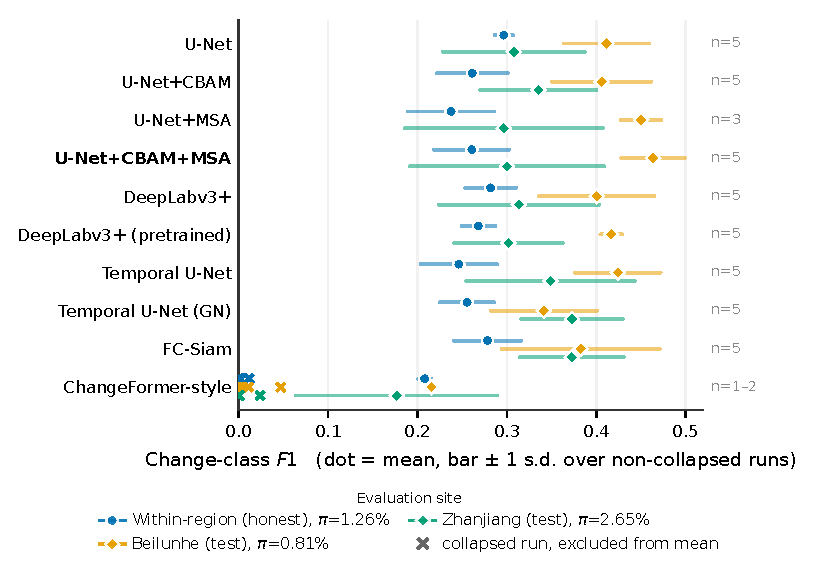
\includegraphics[width=\textwidth]{fig7_cross_region.pdf}
\caption{Per-architecture change $F1$ at the three evaluation sites, uniform
weighting. Each architecture occupies one row and each evaluation site one
sub-row. The three test sets carry different change
prevalence ($\pi = 1.26\%$, $0.81\%$ and $2.65\%$, shown in the key). Symbols are
means and horizontal bars are $\pm 1$ standard deviation over the non-collapsed
run seeds, with $n$ given at the right; runs that collapsed
(change $F1 < 0.05$, drawn as a cross) are excluded from the means and bars.}
\label{fig:crossregion}
\end{figure}

\subsection{The Identification Boundary}
\label{sec:boundary}

The overlap-free control at reduced geometry ($128$\,px, matched prevalence,
zero pixel overlap in both arms) returns $+0.1$\,pp on $F1$ and $-0.3$\,pp on
ROC-AUC (effective $n{=}5$; MDE at $80\%$ power ${\approx}14$\,pp;
Table~\ref{tab:e3c}). This localises the headline gap to the joint spatial
configuration of training and test samples rather than to prevalence or model
capacity alone, but it does not decompose overlap from proximity within that
configuration. A higher-powered overlap-free control with preregistered
independent regions is required to resolve smaller effects.

A leave-one-cluster-out analysis (E6) drops each $1024$-px spatial cell in turn:
across the ten models, removing a single cell moves regional change-$F1$ by as
much as $-30.0$\,pp (Beilunhe), $-20.6$\,pp (Zhanjiang) and $-12.6$\,pp
(Vietnam) in the worst-affected model. Regional point estimates therefore rest
on a handful of spatial clusters, which is why every regional number is reported
as a paired contrast between two arms scored on the same clusters.

Three scope limits apply. (i)~No architecture ranking
(Section~\ref{sec:rand}). (ii)~No field-accuracy claim
(Section~\ref{sec:limitations}). (iii)~The two epochs have unmatched tidal compositions; part of
the measured $t_1$--$t_2$ difference may be water level rather than vegetation.

\subsection{A Benchmarking Checklist}
\label{sec:checklist}

The nearest thing this study has to a generalisable methodological output is a
reporting checklist for change-detection results on spatially
structured imagery. The four items that bear directly on whether the
headline number here is interpretable are: report train--test footprint overlap
as a count (Section~\ref{sec:geom}); include an overlap-free interleaved
control and report its interval width and design size, not only its sign
(Section~\ref{sec:e3}); report the number of independent spatial units and
calibrate the inferential language to it (Section~\ref{sec:limitations}); and
report the class prevalence of every evaluation set, separating prevalence
arithmetic from the case-mix effect (Section~\ref{sec:prevalence}). The list is
derived from this study's confounds; it is a reporting aid for spatially
structured change-detection evaluation.

\subsection{Limitations}
\label{sec:limitations}

\emph{No field reference.} Every number here is agreement with a GMW label, not
accuracy. The designed 2{,}400-point interpretation set has no point
field-interpreted, so no accuracy claim is available.

\emph{Checkpoint-selection channel in the interleaved arm.} Because the
interleaved arm draws its validation and test patches from the same pool,
85\% of its test patches are adjacent to or overlap a validation patch
(Section~\ref{sec:rand}), so validation-based early stopping is spatially
proximate to the test set and can select for it. This is a property of the
interleaved protocol, not a separately controlled confound: the gap reported
for that arm is the total cost of the protocol, including the selection
component. We have not isolated the selection component from the spatial
representation component---a fixed-epoch control (stopping both arms at the
honest arm's median epoch, removing the val-selected stopping rule) would
bound it, and is deferred to a follow-up. The near-zero training-side component
($\Delta_{\mathrm{train}}$) is, if anything, conservative under this channel,
because the channel inflates the interleaved arm's score; the test-side and
interaction components are inflated in the same direction and are not
separable into spatial and selection parts with the current runs.

\emph{Reference-error $\times$ tested-pixel-distribution interaction.} The
protocol contrast is measured against GMW labels on both arms. GMW's label
errors concentrate in the 30\,m fringe band (Section~\ref{sec:labels}), and the
two arms test spatially different pixel sets (the interleaved arm carries
$2.68\times$ the change prevalence and hugs the training fringe). A
reference-error $\times$ tested-pixel-distribution interaction could therefore
contribute part of the TPR shift. The prevalence reweighting holds labels
fixed and is blind to this channel. The channel is bounded by its fringe-band
composition: $89.8\%$ of the honest arm's change pixels and $82.3\%$ of the
interleaved arm's lie within the 30\,m fringe band, a $7.5$\,pp difference in
fringe exposure, the honest arm being the more fringe-exposed
(Section~\ref{app:cm}). This is a composition diagnostic, not an error rate: it
locates where each arm's change pixels sit relative to GMW's unreliable band,
but it bounds neither the direction nor the magnitude of the reference error in
either arm. Because the honest arm is the more fringe-exposed, a reference error
concentrated in that band acts on it at least as strongly as on the interleaved
arm; depending on the sign of the fringe label error it could either lower or
raise the honest arm's agreement, so the channel can enlarge or shrink the gap
and is not identifiable from composition alone. A direct label-noise
sensitivity bounds it (Table~\ref{tab:labelnoise}). Holding the model fixed and
perturbing only the GMW change label, the gap is stable under simulated fringe
error: omitting $20\%$ or $40\%$ of the fringe-band change labels moves it by
$0.8$--$1.7$\,pp ($+28.9$\,pp and $+28.0$\,pp against the $+29.7$\,pp
full-label baseline), and symmetric $20\%$ fringe label noise raises it
($+31.5$\,pp). The inflation is therefore not produced by the interleaved arm
testing noisier labels. Removing the $30$\,m band entirely lowers the gap to
$+19.4$\,pp---nine of the ten models keep $+19$ to $+25$\,pp on the interior
pixels alone, and the tenth (ChangeFormer) turns to $-0.05$\,pp---so roughly a
third of the gap sits in the boundary band where change occurs, a localization
rather than a reference-error artefact.

\begin{table}[H]
\centering
\caption{Label-noise sensitivity of the change-$F1$ gap (interleaved minus
honest, ten architectures pooled, model held fixed). Perturbations act only on
the GMW change label within the $30$\,m fringe band; the model and its
predictions are unchanged.}
\label{tab:labelnoise}
\begin{tabular}{lr}
\toprule
GMW change label & Gap (pp) \\
\midrule
full label (baseline) & $+29.7$ \\
$30$\,m fringe band excluded & $+19.4$ \\
omit $20\%$ of fringe change & $+28.9$ \\
omit $40\%$ of fringe change & $+28.0$ \\
flip $20\%$ of fringe labels & $+31.5$ \\
\bottomrule
\end{tabular}
\end{table}

\emph{Small spatial units.} The test patches form 4, 5 and 2 spatial cell
clusters. No significance test on cross-regional differences is interpretable.

\emph{Correlated split replicates.} The ten-partition replication
(Section~\ref{sec:rand}, Table~\ref{tab:partitions}) establishes that the
interleaving gap is positive in all ten partitions drawn, but the partitions are
not spatially independent: the eligible pool holds only $\sim\!60$ patches, so
any two partitions share $57.5$--$75\%$ of their 40 training patches. The
partition-level 95\% interval ($+26.9$ to $+32.2$\,pp) is therefore a measure
of partition-sampling variability within one region, not a calibrated confidence
interval over independent regions, and it should not be read as evidence that the gap
would replicate unchanged on a different set of sites. Confirming spatial
transfer of the magnitude would require genuinely disjoint regions, which the
present design does not provide.

\emph{Overlap mechanism not identified.} The overlap-free control at reduced
scale ($128$\,px) does not reproduce the headline inflation ($+0.1$\,pp,
percentile spread $[-3.1$, $+3.4]$, descriptive min--max $[-28.5$, $+32.3]$); whether it would at the original
$512$\,px geometry is unresolved. The $2\times2$ factorial separates a small
prevalence-arithmetic component ($+2.7$\,pp) from the dominant
joint-spatial-configuration contrast (TPR shift $+29.6$\,pp), but not
overlap from proximity within the latter.

\emph{Preprocessing confounds.} The SCL mask retains cloud-shadow classes on
the fringe pixels where the signal lives. A strict-mask sensitivity (SCL 4--6
only) shows the inflation is unchanged. The two epochs have unmatched tidal
compositions; at Zhanjiang the mean stable-mangrove $\Delta$NDWI is
$-0.058$ and $55\%$ of stable pixels exceed a $0.05$ threshold, a drift floor
comparable to the change signal that any classifier threshold must exceed.

\section{Conclusions}

A validation score is produced by the model under a sampling and scoring
protocol, not by the model alone. This was demonstrated in the hardest case
for bi-temporal change detection: Sentinel-2 composites, one noisy reference,
change extremely rare ($0.8$--$2.6\%$), training in Vietnam, testing without
fine-tuning on two disjoint Chinese sites. Three conclusions survive the
available evidence.

First (empirical finding): spatially interleaved and buffer-separated
evaluation produce a $+29.6$\,pp difference in rare-change $F1$
($26.9$--$34.1$\,pp across the three split draws) under an identical recipe
and the same 60-patch pool, with only the split assignment varying. The same runs differ by only
$+1.9$\,pp in ROC-AUC (and $+12.5$\,pp in balanced accuracy, an intermediate
anchor between the two), indicating that global pairwise ranking is largely
unchanged, though average precision shifts by $+33.7$\,pp, and exact
prevalence correction (evaluating the PR curve at the target prevalence)
leaves a $+15.2$\,pp high-precision-region advantage for the interleaved
arm (Section~\ref{sec:metric}). The $F1$ contrast is dominated by a $2.5\times$ recall shift under
the four-class argmax decision (TPR $0.19\!\to\!0.48$, FPR $0.002\!\to\!0.007$),
concentrated in the low-FPR operating region. The factorial shows this is a
joint training$\times$test spatial configuration effect: on the $F1$ scale of
Table~\ref{tab:factorial}, changing the test assignment alone contributes
$+5.8$ to $+11.4$\,pp, changing the training assignment alone contributes
$-0.8$ to $+5.1$\,pp, and the interaction exceeds either main effect
($+17.8$ to $+26.1$\,pp of the $+29.2$ to $+32.0$\,pp test-side total). This is
not a simple calibration shift but a configuration-dependent operating-point
effect. Prevalence arithmetic alone contributes
only $+2.7$\,pp. The finding is a thresholded,
recall-driven effect on $F1$; global pairwise ranking (ROC-AUC $+1.9$\,pp)
is largely unchanged, but the high-precision-region ranking itself shifts ($+15.2$\,pp at matched prevalence).

Second (measurement diagnosis): a direct prevalence reweighting isolates a
small prevalence-arithmetic component ($+2.7$\,pp, range $+0.8$--$+3.4$);
the dominant component ($+29.6$\,pp) is the TPR shift at the fixed threshold,
associated with the joint spatial configuration of training and test samples.
This configuration bundles overlap, proximity, and morphology into a single
factor; the design does not permit further decomposition.

Third (identification boundary): a matched-prevalence, zero-overlap control at
reduced patch geometry ($128$\,px) was underpowered to resolve the overlap
mechanism---resubstitution shows no detectable generalisation gap, so the
control is unlikely to be sensitive to memorisation. The reduced-scale block
control is negative in $12$ of the $13$ feasible splits, but its magnitude is
unidentified. The joint spatial configuration (overlap, proximity, morphology,
local prevalence) remains an unidentified black box at the original
$512$-pixel geometry. This is the boundary of what the design can resolve.

No architecture ranking, no field-accuracy claim (no designed validation point
field-interpreted), and no causal decomposition of the residual
contrast are made. The defensible conclusion is that the split protocol is part of the
measurement: a reported change-detection score is a function of model,
protocol, and reference---not of the model alone.

\appendixstart{} \appendix \section{Supporting tables}\label{app:cm}

The material below supports the data description
(Section~\ref{sec:composites}) and the architecture specification
(Section~\ref{sec:arch}): per-scene acquisition metadata
(Table~\ref{tab:scenes}) and the model specification
(Table~\ref{tab:archspec}).

% ===== AUTO-GENERATED by analysis/make_scene_table.py — do not edit =====
% Sources: results/scene_dates_tides.json

\begin{table}[H]
\centering
\caption{Acquisition summary for the 40 scenes used in the dry-season
composites (Section~\ref{sec:composites}); two scenes per tile-epoch, so CF
(the mangrove-mask clear fraction of the two-scene median) is identical for both
scenes of a tile-epoch by construction. Per-scene CF ranges from 0.744 to 1.000
over the 40 scenes; the Vietnam $t_2$ tiles are the low end, the 2024-12-05
pair the cloudiest (whole-tile clear 0.49--0.71). Tidal state is a coarse lunar-age label (spring:
within 3\,d of new or full moon; mid: within 6\,d; otherwise neap), not a
measured water level.}
\label{tab:scenes}
\small
\begin{tabular}{l l l l l}
\toprule
Region & Epoch & Dates & Tidal states & CF range \\
\midrule
Vietnam & $t_1$ & 2019-12-07, 2019-12-12 & mid, spring & 0.984--1.000 \\
         & $t_2$ & 2024-12-05, 2024-12-20 & mid, mid   & 0.744--0.853 \\
\addlinespace
Beilunhe & $t_1$ & 2019-12-07, 2019-12-12 & mid, spring & 0.960--0.989 \\
         & $t_2$ & 2024-12-05, 2024-12-20 & mid, mid   & 0.977--0.997 \\
\addlinespace
Zhanjiang & $t_1$ & 2019-12-04, 2019-12-14 & neap, spring & 0.964--0.980 \\
          & $t_2$ & 2024-12-07, 2025-01-06 & mid, neap & 1.000--1.000 \\
\bottomrule
\end{tabular}
\end{table}

% ===== END AUTO-GENERATED by analysis/make_scene_table.py =====

% ===== AUTO-GENERATED by analysis/make_supplementary_tables.py — do not edit =====





\begin{table}[H]
\caption{Transformer (ChangeFormer-style) architecture specification.}
\label{tab:archspec}
\begin{adjustwidth}{-\extralength}{0cm}
\small
\begin{tabularx}{\fulllength}{l X}
\toprule
Component & Specification \\
\midrule
Per-date encoder & weight-shared (siamese); each nine-band date is
patch-embedded with 16\,px patches into a $32\times32 = 1024$-token grid
(dim 256, learnable positional embedding) and encoded by four Transformer
blocks (8 heads, MLP ratio 4.0, GELU, pre-normalisation) \\
Change branch & one Transformer block (dim 512, 16 heads) on the concatenated
per-date tokens (2048 tokens) \\
Decoder & four strided ConvTranspose2d stages ($\times$2 per stage;
512$\to$256$\to$64$\to$32$\to$8 channels, BatchNorm + ReLU) and a
$1\times1$ convolution head (4 classes) \\
Parameters & 9.56\,M (U-Net family 2.5--3.2\,M; DeepLabv3+ 19.01\,M) \\
Training & common recipe (batch 8; Adam $10^{-3}$; cosine schedule;
class-weighted CE + soft Dice) \\
\bottomrule
\end{tabularx}
\end{adjustwidth}
\end{table}

% Hand-assembled from data/processed/<region>/metadata.json (class_counts,
% n_patches) -- not auto-generated. Source: results/../data/processed/*/metadata.json
\begin{table}[H]
\small
\caption{Patch and pixel counts. ``Change'' = loss + gain. Pixel counts are
summed over patches and therefore count each 10\,m pixel once per patch that
covers it; because patches overlap 50\% on the extraction grid, they overstate
the distinct area by the duplication factors reported in
Section~\ref{sec:geom} and must not be read as sample sizes.}
\label{tab:data}
\begin{tabular}{lcccc}
\toprule
Region / zone & Patches & Stable mangrove & Change & Stable background \\
\midrule
Vietnam, all zones & 76 & 1.89\,M & 0.57\,M & 17.47\,M \\
\quad train / val / test / buffer & 40/10/10/16 & & & \\
Beilunhe (test) & 18 & 0.42\,M & 0.038\,M & 4.26\,M \\
Zhanjiang (test) & 15 & 0.22\,M & 0.104\,M & 3.61\,M \\
\bottomrule
\end{tabular}
\end{table}

\subsection{Experiment registration (E1--E7)}
\label{app:reg}

Each experiment is internally pre-specified before it is reported: its question, its resampling
unit, what its design can identify, and what it cannot. The ``cannot'' column is
the load-bearing one --- the largest measured effect is also the one with the
most confounded design, and this is where that is admitted. Full design and
confound statements are in the body at the point of use
(Table~\ref{tab:reg}).

\begin{table}[H]
\small
\caption{Experiment registration. ``Can'' and ``cannot'' are the design's
identification limits, not statements of what the result happens to be.}
\label{tab:reg}
\setlength{\tabcolsep}{3pt}
\begin{tabular}{lp{0.15\textwidth}p{0.20\textwidth}p{0.24\textwidth}p{0.24\textwidth}}
\toprule
 & Experiment & Question & Can identify & Cannot identify \\
\midrule
E1 & interleaved vs.\ separated split (the headline). & what does the split arrangement alone cost? & the size and robustness of the protocol contrast, a property of the sampling geometry rather than of any model. & which component of the arrangement produces it. \\
E2 & $2\times2$ train/test spatial factorial. & training side, test side, or interaction? & the sign and rough size of a training-side and a test-side component. & attribute either causally, or separate pixel overlap from residual proximity inside the test-side component (delegated to E3). \\
E3 & overlap-free block-interleaved control. & is shared pixel footprint necessary for the inflation? & whether pure residual proximity, with no shared pixel, suffices to produce an inflation of this size---attempted, but E3-C at reduced patch geometry (128\,px) is underpowered to answer it (no generalisation gap in resubstitution; effective $n{=}5$; observed contrast $+0.1$\,pp, percentile spread $[-3.1$, $+3.4]$). & extrapolate E3-B's reduced block scale to the full protocol; the 16 splits narrow its interval but do not remove the scale mismatch. \\
E4 & distance response under separation. & does a buffer remove dependence, or only overlap? & a descriptive near--far gradient. & a resolved distance effect; a patch random intercept is not identified because distance is patch-constant, and the grid-cell-clustered inference is not significant. \\
E5 & effective-separation sensitivity. & do the separated numbers depend on the exact buffer? & robustness to the val--test gap. & probe train--test proximity at all. \\
E6 & leave-one-cluster-out fragility. & how much of a regional number rests on one place? & the fragility of every regional point estimate. & supply a population-level interval. \\
E7 & label-resolution tolerance sweep. & is the change $F1$ a resolution artefact of scoring a 10\,m prediction against a 30\,m reference? & the scale at which the score is sensitive, which distinguishes a 10\,m displacement effect from a 30\,m resolution effect. & bound the reference's accuracy, which needs an independent sample. \\
\bottomrule
\end{tabular}
\end{table}

\subsection{Reproducibility pointers and full experiment inventory}
\label{app:repro}

Table~\ref{tab:inventory} lists every experiment family executed for this
study, including the two that were superseded or found invalid, which are
retained rather than deleted because the branch history is part of the evidence
for the pre-specified claims. Paths, the preflight lock and the commit are
recorded here rather than in the body text.

% ===== AUTO-GENERATED by analysis/experiment_inventory.py -- do not edit =====
\begin{table}[H]
\small
\caption{Full inventory of every experiment family executed for this study. Counts are result files, not training runs: one metrics file summarises one trained model, and checkpoints under \texttt{*/checkpoints/} are the run-level record. Two families that were superseded or found invalid are retained rather than deleted, because the branch history (E3 generation 1 $\rightarrow$ E3-B; composition penalty v0 $\rightarrow$ v1) is part of the evidence for the pre-specified claims. Source: \texttt{results/experiment\_inventory.json} [\texttt{analysis/experiment\_inventory.py}].}
\label{tab:inventory}
\setlength{\tabcolsep}{3pt}
\begin{tabular}{p{0.29\textwidth}rp{0.51\textwidth}}
\toprule
Experiment family & Result files & Description \\
\midrule
primary separated (I/I) & 50 & buffer-separated within-region protocol, 5 run seeds \\\\
secondary sqrt & 150 & square-root weighting replication of the interleaved sweep \\\\
E1 interleaved sweep & 300 & 10 architectures x 10 split draws x 3 run seeds \\\\
E3-B block-interleaved & 260 & overlap-free control, result files across 19 split IDs x 2 arms (16 stratified splits from the design, plus 3 retained from the repaired generation); the design target was 16 splits x 3 architectures x 2 run seeds x 2 arms \\\\
E3-C full-size overlap-free & 90 & disjoint 128 px pool, 40/10/10, scattered vs separated, prevalence matched \\\\
E2 I/R cell & 75 & isolated training, random test \\\\
E7 label-resolution tolerance & --- & morphological erosion/dilation/open/close of the reference change mask, 0--40 m, 3 regions \\\\
E4 distance response & --- & descriptive near--far gradient under the buffer-separated split; grid-cell-clustered inference not significant \\\\
E5 buffer widths & 18 & val-test buffer 1 / 2 / 4 km \\\\
E6 leave-one-cluster-out & 1 & cluster-level fragility of regional point estimates (leave\_one\_cluster\_out.json), 3 regions, 10 models \\\\
PCC baseline & 6 & post-classification comparison, both weighting schemes \\\\
\midrule
\multicolumn{3}{l}{\emph{superseded or invalid, retained as evidence}} \\
E3 generation 1 & --- & superseded by E3-B: two of its four split seeds resolved to the same test set, leaving three distinct test sets (80 runs) \\
composition penalty v0 & --- & invalid: used the block training pool as the composition control; archived, not deleted \\
\bottomrule
\end{tabular}
\end{table}
%% ===== END AUTO-GENERATED (experiment inventory) =====
{\small\sloppy
Artefacts, with the generating script in brackets. Pre-specified split selection
for the overlap-free control: \texttt{logs/e3b\_selection\_lock.txt}
[\texttt{analysis/e3b\_preflight.py}], including the strata values and the
frozen tie-break seed. Prevalence-comparison metrics of Table~\ref{tab:metrics}:
\texttt{results/prevalence\_roc.json}
[\texttt{analysis/roc\_auc\_prevalence.py}]. Full inventory of executed
experiments: \texttt{results/experiment\_inventory.json}
[\texttt{analysis/experiment\_inventory.py}]. Footprint-overlap audit:
\texttt{analysis/footprint\_overlap.py}. Code and results are deposited at
the repository (see Data Availability Statement).\par}





\dataavailability{Sentinel-2 L2A tiles are public and were accessed through the
AWS Open Data Sentinel-2 L2A COG collection. Global Mangrove Watch v4.1.12
is distributed under a CC-BY 4.0 licence by the GMW Consortium; the
second-source GMW 2020 layer is Zenodo record 12756047.
Everything needed to reproduce the numbers in this paper---the analysis code,
the exact patch index lists and split assignments for every protocol, the
trained model checkpoints, the per-pixel prediction dumps, the derived metric
JSONs, and the scripts that generate every table and figure---is available in the public GitHub repository
\url{https://github.com/hao-feier/split-audit};
 the code base accompanying this submission is the
 \texttt{main} branch of that repository at the time of submission.
The full code base is provided with the submission rather than on
request because the paper's subject is the evaluation protocol: a
reader cannot check a claim about a split without the split itself.
\ \ \textbf{Code availability.} The composite, label, patch,
training, counterfactual and analysis pipelines are versioned in the
project repository accompanying this submission; the environment is
 pinned (PyTorch 2.14.0) and every table in the paper is regenerated
 from the JSONs in the accompanying repository by a single script per table.}
 \acknowledgments{The authors thank the GMW Consortium for the open mangrove
 products.}
 \conflictsofinterest{The authors declare no conflicts of interest.}

%% ------------------------------------------------------- back matter
\authorcontributions{J.Y.: conceptualization, formal analysis, investigation,
methodology, software, validation, writing---original draft, writing---review \&
editing. F.H.: data curation, methodology, software, supervision, visualization,
writing---original draft, writing---review \& editing.}
\funding{This research received no external funding.}
\institutionalreview{Not applicable; no human or animal subjects were involved.}
\informedconsent{Not applicable.}
\abbreviations{Abbreviations}{CD, change detection; GMW, Global Mangrove Watch;
OA, overall accuracy; mIoU, mean intersection over union; $F1_{ch}$ /
$IoU_{ch}$, binary change (loss + gain) F1 / IoU; CBAM, convolutional block
attention module; MSA, multi-scale feature gate; ASPP, atrous spatial pyramid
pooling; SCL, Scene Classification Layer; UTM, Universal Transverse Mercator;
STAC, SpatioTemporal Asset Catalog; CC-BY, Creative Commons Attribution.}

\begin{adjustwidth}{-\extralength}{0cm}
\reftitle{References}
\bibliography{refs}
\end{adjustwidth}

\end{document}
